% design.tex — Matryoshka Tree Design Document
% Compile: pdflatex design.tex  (run twice for ToC/hyperref)

\documentclass[11pt,letterpaper]{article}

% ── Packages ──────────────────────────────────────────────────────
\usepackage[margin=1in]{geometry}
\usepackage{amsmath,amssymb}
\usepackage{booktabs}
\usepackage{graphicx}
\usepackage{hyperref}
\usepackage{fancyhdr}
\usepackage{siunitx}
\usepackage{xcolor}
\usepackage{longtable}
\usepackage{float}
\usepackage{enumitem}
\usepackage{microtype}
\usepackage{tikz}
\usepackage{listings}
\usepackage{tocloft}
\usepackage[font=small,labelfont=bf]{caption}

\usetikzlibrary{
  arrows.meta,
  positioning,
  decorations.pathreplacing,
  calc,
  fit,
  patterns,
  shapes.geometric,
  shapes.multipart,
  backgrounds,
  matrix
}

% ── Colors ────────────────────────────────────────────────────────
\definecolor{inodecolor}{HTML}{DBEAFE}    % light blue — internal nodes
\definecolor{leafcolor}{HTML}{D1FAE5}     % light green — leaf nodes
\definecolor{simdblk}{HTML}{FDE68A}       % gold — SIMD blocks
\definecolor{clblk}{HTML}{C4B5FD}         % violet — cache-line blocks
\definecolor{pageblk}{HTML}{FECACA}       % rose — page blocks
\definecolor{ptrcolor}{HTML}{3B82F6}      % blue — pointers
\definecolor{keycolor}{HTML}{1F2937}      % dark gray — keys
\definecolor{headercolor}{HTML}{F3F4F6}   % light gray — headers
\definecolor{rankcolor}{HTML}{A7F3D0}     % mint — sorted_rank
\definecolor{codebg}{HTML}{F8FAFC}

% ── Listings ──────────────────────────────────────────────────────
\lstset{
  basicstyle=\ttfamily\small,
  backgroundcolor=\color{codebg},
  frame=single,
  framerule=0.4pt,
  rulecolor=\color{gray!40},
  breaklines=true,
  columns=fullflexible,
  keepspaces=true,
  showstringspaces=false,
  language=C,
  morekeywords={int32_t,int16_t,uint8_t,uint16_t,uint32_t,uint64_t,size_t,bool,
                __m128i,mt_inode_t,mt_lnode_t,mt_node_t,mt_cl_leaf_t,
                mt_cl_inode_t,mt_cl_slot_t,mt_page_header_t},
}

% ── Page style ────────────────────────────────────────────────────
\pagestyle{fancy}
\fancyhf{}
\fancyhead[L]{\small Matryoshka Tree Design Document}
\fancyhead[R]{\small\thepage}
\renewcommand{\headrulewidth}{0.4pt}

\hypersetup{
  colorlinks=true,
  linkcolor=blue!60!black,
  citecolor=blue!60!black,
  urlcolor=blue!60!black,
  pdfstartview=FitH,
}
\pdfstringdefDisableCommands{%
  \def\textsuperscript#1{+}%
}

% ── Convenience macros ────────────────────────────────────────────
\newcommand{\Oh}{\mathcal{O}}
\newcommand{\ceil}[1]{\lceil #1 \rceil}
\newcommand{\floor}[1]{\lfloor #1 \rfloor}
\newcommand{\code}[1]{\texttt{#1}}

% ══════════════════════════════════════════════════════════════════
\begin{document}

\begin{titlepage}
\centering
\vspace*{2cm}
{\Huge\bfseries Matryoshka Trees\par}
\vspace{0.5cm}
{\Large\itshape A Cache-Conscious B\textsuperscript{+} Tree with\\
  Matryoshka-Nested Sub-Trees at Every Memory Hierarchy Level\par}
\vspace{2cm}
{\large Design Document\par}
\vspace{1cm}
{\large\today\par}
\vfill
{\small
This document describes the design of the \emph{matryoshka tree}, a B\textsuperscript{+}
tree variant in which each leaf node (a \SI{4}{\kilo\byte} page) contains a complete
B\textsuperscript{+} sub-tree of cache-line-sized (\SI{64}{\byte}) sub-nodes, each
searched via SIMD register--width (\SI{16}{\byte}) comparisons.  This ``matryoshka
nesting''---trees within trees, each level mapped to a memory hierarchy
level---replaces the flat FAST-blocked arrays of the earlier design with a
true hierarchical B\textsuperscript{+} structure at every scale.  Insert and delete
operate on individual cache-line sub-nodes via split, merge, and redistribute,
giving $\Oh(\text{sub\_height} \times 15)$ work per leaf modification instead of
$\Oh(B)$ flat-array rebuilds.  The name reflects the nested Russian-doll
architecture: SIMD registers nest inside cache-line sub-nodes, which form a
B\textsuperscript{+} sub-tree inside each page-sized leaf node, which composes
the full outer B\textsuperscript{+} tree.}
\end{titlepage}

\tableofcontents
\newpage

% ══════════════════════════════════════════════════════════════════
\section{Introduction}
\label{sec:intro}

The matryoshka tree addresses a long-standing tension in main-memory index
design: \emph{search throughput versus modification cost}.

On one end of the spectrum, the FAST tree~\cite{kim2010fast} achieves
near-optimal search throughput by mapping an implicit (pointerless)
search tree onto the memory hierarchy through a recursive blocking
scheme.  Each level of the blocking matches a level of the hardware:
SSE registers (\SI{16}{\byte}), cache lines (\SI{64}{\byte}), pages
(\SI{4}{\kilo\byte}), and superpages (\SI{2}{\mebi\byte}).  Because the
layout is implicit (positions are computed arithmetically, not followed
via pointers), it eliminates pointer-chasing stalls and maximises
hardware prefetch effectiveness.  The price is that any structural
modification---insertion or deletion---requires a full $\Oh(n)$ rebuild.

On the other end, classical B\textsuperscript{+}
trees~\cite{bayer1972organization,comer1979ubiquitous} support
$\Oh(\log_B n)$ modifications via node-local splits and merges, but
suffer from pointer-chasing at every level of the tree, causing a TLB
miss and often an L2/L3 cache miss per node visited.

The original matryoshka design confined FAST-style flat blocked arrays
\emph{within} each B\textsuperscript{+} leaf node.  While this retained
B\textsuperscript{+} tree navigation between nodes, every insertion or
deletion into a leaf still required an $\Oh(B)$ extraction-and-rebuild
of the entire FAST layout (where $B = 511$ for \SI{4}{\kilo\byte}
pages).  The flat layout could not be modified in place.

The current design eliminates this bottleneck.  Instead of a flat
blocked array, each leaf page now contains a genuine B\textsuperscript{+}
\emph{sub-tree} of cache-line-sized sub-nodes.  Insertions and deletions
operate on individual \SI{64}{\byte} sub-nodes---splitting, merging, and
redistributing cache-line leaves and cache-line internal nodes---without
touching the rest of the page.  The result is:

\begin{itemize}[nosep]
  \item \textbf{Fast intra-node search}: Each leaf page contains a
    B\textsuperscript{+} sub-tree of up to 63 cache-line sub-nodes,
    navigated via SIMD-accelerated scans at each sub-tree level.
    A search touches at most $\text{sub\_height} + 1$ cache lines.
  \item \textbf{Efficient per-key modifications}: Insert and delete
    modify only the affected CL leaf (\SI{64}{\byte}, 15 keys max)
    and propagate splits or merges through at most $\text{sub\_height}$
    CL internal levels.  Cost: $\Oh(\text{sub\_height} \times 15)$ per
    leaf modification, versus $\Oh(511)$ for the old flat rebuild.
  \item \textbf{Matryoshka nesting}: The tree is self-similar at every
    scale---a B\textsuperscript{+} tree of pages, each page containing
    a B\textsuperscript{+} tree of cache lines, each cache line
    searched via SIMD registers---mirroring the CPU memory hierarchy.
  \item \textbf{Eager deletion}: Jannink's redistribute/merge algorithm
    operates at both the CL sub-tree level (within a page) and the
    outer B\textsuperscript{+} tree level (between pages), maintaining
    minimum occupancy invariants at every level.
  \item \textbf{Arena allocation}: Leaf pages are co-located within
    \SI{2}{\mebi\byte} arenas.  \code{MAP\_HUGETLB} is attempted;
    on failure, \code{posix\_memalign} with
    \code{madvise(MADV\_HUGEPAGE)} provides transparent huge pages.
  \item \textbf{Range scans}: A doubly-linked leaf list supports
    efficient sequential iteration across pages.
\end{itemize}

\begin{center}
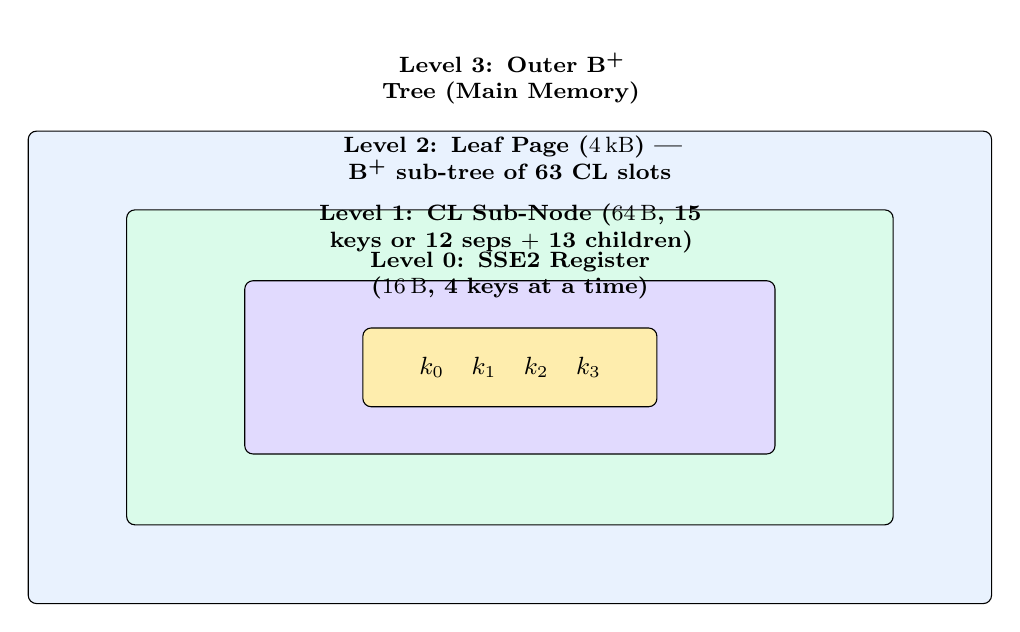
\begin{tikzpicture}[
  every node/.style={draw, rounded corners=3pt, minimum height=1.3cm,
                     text width=5cm, align=center, font=\small},
  level0/.style={fill=simdblk!70},
  level1/.style={fill=clblk!50},
  level2/.style={fill=leafcolor!80},
  level3/.style={fill=inodecolor!60},
  >=stealth
]
  % Outermost: B+ tree
  \node[level3, minimum height=6.0cm, text width=12cm,
        label={[font=\footnotesize\bfseries]above:Level 3: Outer B\textsuperscript{+} Tree (Main Memory)}]
    (bptree) {};

  % Page-level: leaf page with sub-tree
  \node[level2, minimum height=4.0cm, text width=9.5cm,
        label={[font=\footnotesize\bfseries]above:Level 2: Leaf Page (\SI{4}{\kilo\byte})
          --- B\textsuperscript{+} sub-tree of 63 CL slots}]
    at (bptree.center) (page) {};

  % Cache-line level
  \node[level1, minimum height=2.2cm, text width=6.5cm,
        label={[font=\footnotesize\bfseries]above:Level 1: CL Sub-Node (\SI{64}{\byte},
          15 keys or 12 seps $+$ 13 children)}]
    at (page.center) (clblock) {};

  % SIMD level
  \node[level0, minimum height=1.0cm, text width=3.5cm,
        label={[font=\footnotesize\bfseries]above:Level 0: SSE2 Register (\SI{16}{\byte}, 4 keys at a time)}]
    at (clblock.center) (simd) {$k_0\;\; k_1\;\; k_2\;\; k_3$};

\end{tikzpicture}
\captionof{figure}{%
  \textbf{Matryoshka nesting hierarchy.}
  Each level physically nests within the next.
  SIMD registers (\textbf{Level~0}, gold) scan within cache-line
  sub-nodes (\textbf{Level~1}, violet), which form a B\textsuperscript{+}
  sub-tree inside each page-sized leaf (\textbf{Level~2}, green),
  composing the full outer B\textsuperscript{+} tree (\textbf{Level~3}, blue).
  Within each page, navigation uses slot indices (1--63); between
  pages, navigation uses explicit child pointers.}
\label{fig:nesting}
\end{center}


% ══════════════════════════════════════════════════════════════════
\section{Conceptual Motivations}
\label{sec:concepts}

\subsection{Matryoshka Dolls}

The project is named after Russian \emph{matryoshka} (nesting) dolls---a
set of hollow wooden figures of decreasing size, each placed inside the
next larger one.  When you open the outermost doll, you find a slightly
smaller doll inside; open that, and there is a yet smaller one, and so
on down to the smallest solid figure at the centre.

The tree structure mirrors this physical nesting precisely.  The outermost
``doll'' is the B\textsuperscript{+} tree itself, navigated via pointers
in main memory.  Open a leaf page---the next doll---and inside you find
not a flat array but a complete B\textsuperscript{+} sub-tree of
cache-line-sized nodes.  Open a cache-line sub-node---a still smaller
doll---and its sorted keys are searched via SSE2 register--width
comparisons, four keys at a time.

\begin{center}
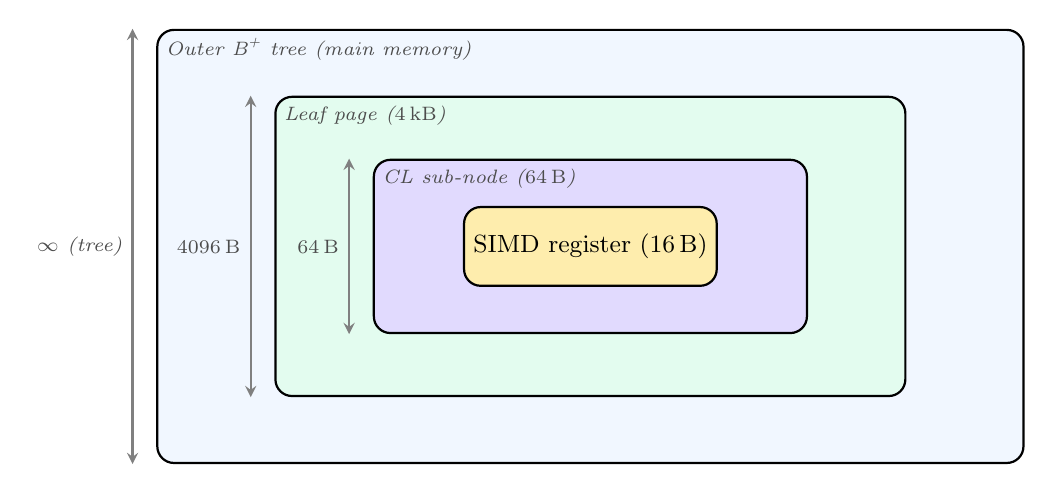
\begin{tikzpicture}[
  doll/.style={draw, thick, rounded corners=6pt, align=center, font=\small},
  >=stealth,
  lbl/.style={font=\scriptsize\itshape, text=gray!60!black},
]
  % Outermost doll
  \node[doll, fill=inodecolor!40, minimum width=11cm, minimum height=5.5cm] (d3) {};
  \node[lbl, anchor=north west] at (d3.north west) {Outer B\textsuperscript{+} tree (main memory)};

  % Second doll
  \node[doll, fill=leafcolor!60, minimum width=8cm, minimum height=3.8cm] at (d3.center) (d2) {};
  \node[lbl, anchor=north west] at (d2.north west) {Leaf page (\SI{4}{\kilo\byte})};

  % Third doll
  \node[doll, fill=clblk!50, minimum width=5.5cm, minimum height=2.2cm] at (d2.center) (d1) {};
  \node[lbl, anchor=north west] at (d1.north west) {CL sub-node (\SI{64}{\byte})};

  % Innermost doll
  \node[doll, fill=simdblk!70, minimum width=3cm, minimum height=1.0cm] at (d1.center) (d0) {SIMD register (\SI{16}{\byte})};

  % Size annotations
  \draw[<->, thick, gray] ([xshift=-0.3cm]d3.south west) -- ([xshift=-0.3cm]d3.north west)
    node[midway, left, lbl] {$\infty$ (tree)};
  \draw[<->, thick, gray] ([xshift=-0.3cm]d2.south west) -- ([xshift=-0.3cm]d2.north west)
    node[midway, left, lbl] {\SI{4096}{\byte}};
  \draw[<->, thick, gray] ([xshift=-0.3cm]d1.south west) -- ([xshift=-0.3cm]d1.north west)
    node[midway, left, lbl] {\SI{64}{\byte}};
\end{tikzpicture}
\captionof{figure}{%
  \textbf{The matryoshka doll analogy.}
  Each level of the data structure physically nests within the next
  larger one, just as each wooden doll nests within its larger shell.}
\label{fig:dolls}
\end{center}

Each level nests \emph{physically} within the next: every CL sub-node
resides within a page, and every SIMD comparison operates on bytes
within a CL sub-node.  The analogy is not merely decorative---it
captures the essential design principle.  Just as a matryoshka set
is a single unified artefact despite comprising multiple nested objects,
the matryoshka tree is a single coherent index despite operating under
different structural rules at each nesting level.

\subsection{Inception Analogy}

The nesting also evokes Christopher Nolan's film \emph{Inception}
(2010), whose premise involved dreams nested within dreams to great
depth, each level operating under its own rules and timescale.

In the matryoshka tree, each nesting level operates under its own
structural rules:

\begin{itemize}[nosep]
  \item The \textbf{outer B\textsuperscript{+} tree} uses pointers and
    page-granularity splits.  Its branching factor is up to 340 children.
  \item The \textbf{CL sub-tree} within each page uses slot indices
    (1--63) and cache-line-granularity split, merge, and redistribute
    operations.  CL leaves hold 15 keys; CL internal nodes hold 12
    separators and 13 children.
  \item \textbf{SIMD search} operates on register-width vectors,
    comparing 4 keys per instruction in a sorted scan.
\end{itemize}

The increasing time compression in deeper dream levels in
\emph{Inception} parallels the decreasing access latency at deeper
nesting levels in the matryoshka tree: main memory access takes
${\sim}\SI{100}{\nano\second}$, L1 cache hits take
${\sim}\SI{1}{\nano\second}$, and register operations complete in a
fraction of a nanosecond.  Each level inward is both physically smaller
and faster, just as each dream level inward compressed subjective time.

However, unlike \emph{Inception}'s concern with subjective reality and
the instability of deeply nested dream states, the matryoshka tree's
nesting is structurally stable.  Each level reinforces the others
through well-defined split/merge invariants: a CL leaf split propagates
to its CL internal parent; if the page runs out of CL slots, a page-level
split propagates to the outer B\textsuperscript{+} tree.  The nesting
never ``collapses''---it is the foundation of correctness, not a source
of fragility.


% ══════════════════════════════════════════════════════════════════
\section{Related Work}
\label{sec:related}

The matryoshka tree draws from several lines of research in cache-conscious
indexing.  We situate it within the literature below.

\paragraph{B-trees and B\textsuperscript{+} trees.}
Bayer and McCreight~\cite{bayer1972organization} introduced the B-tree as a
balanced, external-memory search tree with $\Oh(\log_B n)$ search and
modification costs.  The B\textsuperscript{+} tree variant, formalized in
surveys by Comer~\cite{comer1979ubiquitous} and later by
Graefe~\cite{graefe2011modern}, stores all data in leaf nodes connected by a
linked list, with internal nodes serving purely as a routing index.  This
separation enables efficient range scans and simplifies concurrency
control~\cite{lehman1981efficient}.

\paragraph{Cache-sensitive search trees (CSS-trees).}
Rao and Ross~\cite{rao1999cache} observed that the pointer overhead in
B\textsuperscript{+} trees wastes cache space and proposed \emph{CSS-trees}:
implicit directory levels stored in sorted arrays, with child offsets computed
arithmetically.  This eliminates pointers within the directory, improving cache
utilization.  However, CSS-trees are static (read-only after bulk construction).

\paragraph{Cache-conscious B\textsuperscript{+} trees (CSB\textsuperscript{+}-trees).}
Rao and Ross~\cite{rao2000making} extended their cache-conscious approach to
support modifications by storing child nodes of each internal node in a
contiguous array, so a single pointer suffices per node (plus an offset).
This halves pointer storage compared to standard B\textsuperscript{+} trees.
Hankins and Patel~\cite{hankins2003effect} subsequently showed that the
optimal node size for cache-conscious B\textsuperscript{+} trees is
typically the cache-line size or a small multiple thereof, depending on the
access pattern.

\paragraph{SIMD-accelerated search.}
Zhou and Ross~\cite{zhou2002implementing} demonstrated that SIMD instructions
(specifically SSE2's \code{\_mm\_cmpgt\_epi32}) could accelerate database
operations including sorted-array search, achieving 4$\times$ parallelism per
comparison.  Schlegel et al.~\cite{schlegel2009kary} generalized this to
$k$-ary search on modern processors, showing that $k = 2^{d_K}$ simultaneous
comparisons reduce tree depth by a factor of $d_K$ relative to binary search.

\paragraph{FAST: Fast Architecture Sensitive Tree.}
Kim et al.~\cite{kim2010fast} combined hierarchical blocking with SIMD
comparisons to build a static index that maps directly onto the memory hierarchy.
The FAST tree defines blocking depths $d_K$ (SIMD register), $d_L$ (cache line),
and $d_P$ (page/superpage) such that each block fits exactly in the
corresponding hardware unit.  Within each block, keys are stored in BFS
(breadth-first search) order of a complete binary tree, enabling SIMD-parallel
comparisons at each level.  The FAST tree achieves throughput within a factor of
two of a hardware-optimal binary search, but requires $\Oh(n)$ reconstruction
for any modification.

\paragraph{Masstree.}
Mao et al.~\cite{mao2012cache} built Masstree, a trie of B\textsuperscript{+}
trees designed for concurrent multicore key-value stores.  Each
B\textsuperscript{+} tree level handles a fixed-width slice of the key,
amortizing cache misses across key bytes.  Masstree uses optimistic concurrency
(version numbers per node) rather than locking, achieving high throughput under
contention.  Like the matryoshka tree, Masstree nests simpler structures inside
larger ones, though it uses a trie/B-tree nesting rather than
sub-tree/B-tree nesting.

\paragraph{Adaptive Radix Tree (ART).}
Leis et al.~\cite{leis2013adaptive} proposed ART, which adaptively selects
among four node sizes (4, 16, 48, 256 children) to balance space and search
efficiency.  ART uses SIMD for its smallest node type (Node16, using
\code{\_mm\_cmpeq\_epi8} for 16-way key matching).  While ART excels for
variable-length string keys, the matryoshka tree targets fixed-size integer
keys where cache-line-granularity B\textsuperscript{+} operations are most
effective.

\paragraph{Positioning of the matryoshka tree.}
The matryoshka tree occupies a specific niche: it provides SIMD-accelerated
intra-page search while supporting per-key modifications that touch only
the affected cache-line sub-nodes, avoiding the $\Oh(B)$ rebuild cost of
FAST-within-B\textsuperscript{+} designs and the $\Oh(n)$ rebuild cost
of pure FAST.  Table~\ref{tab:comparison} summarises the trade-offs.

\begin{table}[H]
\centering
\caption{\textbf{Comparison of index structures for sorted integer keys.}
  $n$ = number of keys, $B$ = node capacity, $h$ = sub-tree height
  within a leaf.}
\label{tab:comparison}
\small
\begin{tabular}{@{}lcccc@{}}
\toprule
\textbf{Structure} & \textbf{Search} & \textbf{Insert/Delete} & \textbf{Range Scan} & \textbf{SIMD} \\
\midrule
B\textsuperscript{+}-tree~\cite{bayer1972organization}
  & $\Oh(\log_B n)$ & $\Oh(\log_B n)$ & linked list & no \\
CSS-tree~\cite{rao1999cache}
  & $\Oh(\log_2 n)$ & $\Oh(n)$ rebuild & scan & no \\
CSB\textsuperscript{+}-tree~\cite{rao2000making}
  & $\Oh(\log_B n)$ & $\Oh(\log_B n)$ & linked list & no \\
FAST~\cite{kim2010fast}
  & $\Oh(\log_2 n / d_K)$ & $\Oh(n)$ rebuild & scan & yes \\
ART~\cite{leis2013adaptive}
  & $\Oh(k)$ depth & $\Oh(k)$ depth & DFS & partial \\
Masstree~\cite{mao2012cache}
  & $\Oh(k/w \cdot \log_B n)$ & $\Oh(k/w \cdot \log_B n)$ & linked list & no \\
\textbf{Matryoshka}
  & $\Oh(\log_B n + h)$ & $\Oh(h \cdot b + \log_B n)$ & linked list & yes \\
\bottomrule
\end{tabular}
\end{table}

\noindent
In the table above, $h$ denotes the sub-tree height within a leaf
page (typically 0--2) and $b$ denotes the CL sub-node capacity (15 keys
for CL leaves, 12 separators for CL internals).


% ══════════════════════════════════════════════════════════════════
\section{Architecture Overview}
\label{sec:architecture}

A matryoshka tree is a B\textsuperscript{+} tree with two node types.
The distinguishing feature is that leaf nodes are not flat arrays of keys
but instead contain a nested B\textsuperscript{+} sub-tree of
cache-line-sized sub-nodes:

\begin{description}[leftmargin=2em, labelindent=0em]
  \item[Internal nodes] store sorted keys and child pointers in a
    conventional B\textsuperscript{+} layout.  Intra-node search uses
    SIMD-accelerated linear scan (for small fanout) or binary search
    (for large fanout).  Each internal node fits in one \SI{4}{\kilo\byte}
    page, holding up to 339 keys and 340 child pointers.

  \item[Leaf nodes] are \SI{4}{\kilo\byte} pages divided into 64
    cache-line-sized (\SI{64}{\byte}) slots.  Slot~0 is a page header.
    Slots~1--63 hold CL sub-nodes---either \emph{CL leaves} (sorted
    arrays of up to 15 \code{int32\_t} keys) or \emph{CL internals}
    (separator keys and child slot indices).  These sub-nodes form a
    B\textsuperscript{+} sub-tree within the page.  Leaves are doubly
    linked for range scans.
\end{description}

\subsection{Memory Hierarchy Mapping}

Each level of the matryoshka nesting corresponds to a level of the CPU
memory hierarchy:

\begin{table}[H]
\centering
\caption{\textbf{Memory hierarchy mapping.}  Each nesting level is sized
  to match a hardware unit.}
\label{tab:hierarchy}
\small
\begin{tabular}{@{}clll@{}}
\toprule
\textbf{Level} & \textbf{Hardware Unit} & \textbf{Size} & \textbf{Role in Matryoshka Tree} \\
\midrule
0 & SSE2 register  & \SI{16}{\byte}         & SIMD scan: 4 keys per comparison \\
1 & Cache line      & \SI{64}{\byte}         & CL sub-node: 15 keys (leaf) or 12 seps $+$ 13 children (internal) \\
2 & Page            & \SI{4}{\kilo\byte}     & Leaf page: B\textsuperscript{+} sub-tree of 63 CL slots \\
3 & Main memory     & $\infty$               & Outer B\textsuperscript{+} tree: pointer-based navigation \\
\bottomrule
\end{tabular}
\end{table}

The key insight is that the structure is \emph{self-similar} at each level:
the outer tree is a B\textsuperscript{+} tree of pages, and each page
internally contains a B\textsuperscript{+} tree of cache lines.  At the
finest granularity, each sorted cache-line array is searched by scanning
4~keys at a time in an SSE2 register.  This recursive B\textsuperscript{+}
structure at every scale is what distinguishes the matryoshka design from
approaches that use a flat array or implicit tree within each node.

\subsection{Overall Tree Structure}

Figure~\ref{fig:tree-structure} shows the complete tree structure,
from the outer B\textsuperscript{+} tree down through the CL sub-tree
within each leaf page.

\begin{figure}[H]
\centering
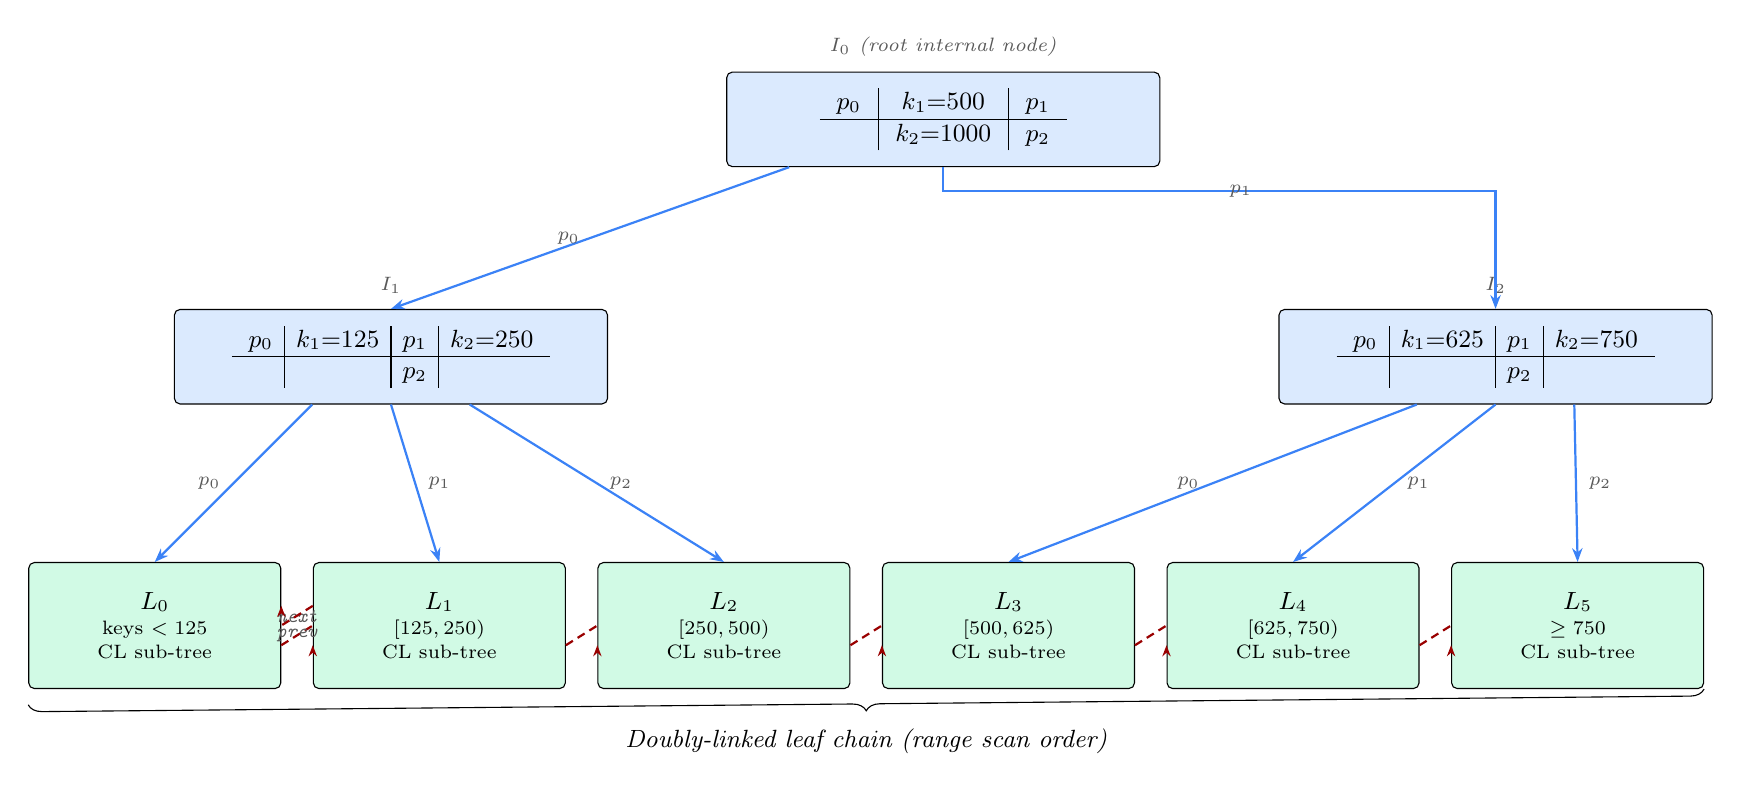
\begin{tikzpicture}[
  inode/.style={
    draw, fill=inodecolor, rounded corners=2pt,
    minimum width=5.5cm, minimum height=1.2cm,
    font=\small
  },
  leaf/.style={
    draw, fill=leafcolor, rounded corners=2pt,
    minimum width=3.2cm, minimum height=1.6cm,
    font=\small, align=center
  },
  ptr/.style={-{Stealth[length=5pt]}, thick, ptrcolor},
  leaflink/.style={-{Stealth[length=4pt]}, thick, red!60!black, densely dashed},
  lbl/.style={font=\scriptsize\itshape, text=gray!70!black}
]

  % ── Root internal node ──
  \node[inode] (root) {%
    \begin{tabular}{c@{\hskip 6pt}|@{\hskip 6pt}c@{\hskip 6pt}|@{\hskip 6pt}c}
      $p_0$ & $k_1{=}500$ & $p_1$ \\
      \hline
      & $k_2{=}1000$ & $p_2$ \\
    \end{tabular}
  };
  \node[lbl, above=2pt of root] {$I_0$ (root internal node)};

  % ── Child internal nodes ──
  \node[inode, below left=1.8cm and 1.5cm of root] (i1) {%
    \begin{tabular}{c@{\hskip 4pt}|@{\hskip 4pt}c@{\hskip 4pt}|@{\hskip 4pt}c@{\hskip 4pt}|@{\hskip 4pt}c}
      $p_0$ & $k_1{=}125$ & $p_1$ & $k_2{=}250$ \\
      \hline
      & & $p_2$ & \\
    \end{tabular}
  };
  \node[lbl, above=2pt of i1] {$I_1$};

  \node[inode, below right=1.8cm and 1.5cm of root] (i2) {%
    \begin{tabular}{c@{\hskip 4pt}|@{\hskip 4pt}c@{\hskip 4pt}|@{\hskip 4pt}c@{\hskip 4pt}|@{\hskip 4pt}c}
      $p_0$ & $k_1{=}625$ & $p_1$ & $k_2{=}750$ \\
      \hline
      & & $p_2$ & \\
    \end{tabular}
  };
  \node[lbl, above=2pt of i2] {$I_2$};

  % ── Leaf nodes ──
  \node[leaf, below=2.0cm of i1, xshift=-3.0cm] (l0)
    {$L_0$\\[-2pt]{\scriptsize keys $< 125$}\\[-2pt]{\scriptsize CL sub-tree}};
  \node[leaf, right=0.4cm of l0] (l1)
    {$L_1$\\[-2pt]{\scriptsize $[125, 250)$}\\[-2pt]{\scriptsize CL sub-tree}};
  \node[leaf, right=0.4cm of l1] (l2)
    {$L_2$\\[-2pt]{\scriptsize $[250, 500)$}\\[-2pt]{\scriptsize CL sub-tree}};
  \node[leaf, right=0.4cm of l2] (l3)
    {$L_3$\\[-2pt]{\scriptsize $[500, 625)$}\\[-2pt]{\scriptsize CL sub-tree}};
  \node[leaf, right=0.4cm of l3] (l4)
    {$L_4$\\[-2pt]{\scriptsize $[625, 750)$}\\[-2pt]{\scriptsize CL sub-tree}};
  \node[leaf, right=0.4cm of l4] (l5)
    {$L_5$\\[-2pt]{\scriptsize $\geq 750$}\\[-2pt]{\scriptsize CL sub-tree}};

  % ── Pointers: root → children ──
  \draw[ptr] (root.south west) ++(0.8cm, 0) -- (i1.north) node[midway, lbl, left] {$p_0$};
  \draw[ptr] (root.south) -- ++(0,-0.3cm) -| (i2.north) node[near start, lbl, right] {$p_1$};

  % ── Pointers: I1 → leaves ──
  \draw[ptr] (i1.south) ++(-1.0cm, 0) -- (l0.north) node[midway, lbl, left=1pt] {$p_0$};
  \draw[ptr] (i1.south) -- (l1.north) node[midway, lbl, right=1pt] {$p_1$};
  \draw[ptr] (i1.south) ++(1.0cm, 0) -- (l2.north) node[midway, lbl, right=1pt] {$p_2$};

  % ── Pointers: I2 → leaves ──
  \draw[ptr] (i2.south) ++(-1.0cm, 0) -- (l3.north) node[midway, lbl, left=1pt] {$p_0$};
  \draw[ptr] (i2.south) -- (l4.north) node[midway, lbl, right=1pt] {$p_1$};
  \draw[ptr] (i2.south) ++(1.0cm, 0) -- (l5.north) node[midway, lbl, right=1pt] {$p_2$};

  % ── Leaf linked list ──
  \draw[leaflink] (l0.east) ++(0, -0.25cm) -- (l1.west |- l0.east) ++(0, -0.25cm)
    node[midway, lbl, above=1pt] {\code{next}};
  \draw[leaflink] (l1.east) ++(0, -0.25cm) -- (l2.west |- l1.east) ++(0, -0.25cm);
  \draw[leaflink] (l2.east) ++(0, -0.25cm) -- (l3.west |- l2.east) ++(0, -0.25cm);
  \draw[leaflink] (l3.east) ++(0, -0.25cm) -- (l4.west |- l3.east) ++(0, -0.25cm);
  \draw[leaflink] (l4.east) ++(0, -0.25cm) -- (l5.west |- l4.east) ++(0, -0.25cm);

  % ── prev pointer (example) ──
  \draw[leaflink] (l1.west) ++(0, 0.25cm) -- (l0.east |- l1.west) ++(0, 0.25cm)
    node[midway, lbl, below=1pt] {\code{prev}};

  % ── Brace labels ──
  \draw[decorate, decoration={brace, amplitude=5pt, mirror}]
    (l0.south west) ++(0,-0.2cm) -- (l5.south east |- l0.south west) ++(0,-0.2cm)
    node[midway, below=8pt, font=\small\itshape] {Doubly-linked leaf chain (range scan order)};

\end{tikzpicture}
\caption{\textbf{Overall matryoshka tree structure.}
  Internal nodes $I_0$--$I_2$ (blue) contain sorted separator keys
  and child pointers.  Leaf nodes $L_0$--$L_5$ (green) each contain a
  B\textsuperscript{+} sub-tree of CL sub-nodes (not a flat array).
  Red dashed arrows show the doubly-linked leaf list; blue solid arrows
  show child pointers.}
\label{fig:tree-structure}
\end{figure}


% ══════════════════════════════════════════════════════════════════
\section{Node Structures}
\label{sec:nodes}

\subsection{CL Leaf Sub-Node (\code{mt\_cl\_leaf\_t})}
\label{sec:cl-leaf}

A cache-line leaf stores a sorted array of up to 15 \code{int32\_t} keys
in exactly \SI{64}{\byte}:

\begin{figure}[H]
\centering
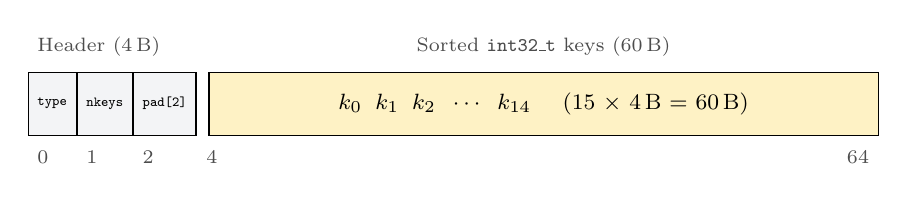
\begin{tikzpicture}[
  box/.style={draw, minimum height=0.8cm, font=\footnotesize, anchor=west},
  lbl/.style={font=\scriptsize, text=gray!60!black},
]
  \node[box, fill=headercolor, minimum width=0.5cm] (type) at (0,0) {\tiny\code{type}};
  \node[box, fill=headercolor, minimum width=0.6cm, right=0pt of type] (nk) {\tiny\code{nkeys}};
  \node[box, fill=headercolor, minimum width=0.7cm, right=0pt of nk] (pad) {\tiny\code{pad[2]}};
  \node[box, fill=simdblk!50, minimum width=8.5cm, right=0.15cm of pad] (keys)
    {$k_0 \;\; k_1 \;\; k_2 \;\; \cdots \;\; k_{14}$ \quad (15 $\times$ \SI{4}{\byte} = \SI{60}{\byte})};

  % Byte offsets
  \node[lbl, below=2pt of type.south west, anchor=north west] {0};
  \node[lbl, below=2pt of type.south east, anchor=north west] {1};
  \node[lbl, below=2pt of nk.south east, anchor=north west] {2};
  \node[lbl, below=2pt of pad.south east, anchor=north west] {4};
  \node[lbl, below=2pt of keys.south east, anchor=north east] {64};

  % Labels
  \node[lbl, above=2pt of type.north west, anchor=south west] {Header (\SI{4}{\byte})};
  \node[lbl, above=2pt of keys.north, anchor=south] {Sorted \code{int32\_t} keys (\SI{60}{\byte})};
\end{tikzpicture}
\caption{\textbf{CL leaf sub-node layout (\code{mt\_cl\_leaf\_t}, \SI{64}{\byte}).}
  \code{type} = \code{MT\_CL\_LEAF} (1 byte), \code{nkeys} = number of
  valid keys (1 byte), 2 bytes padding, then up to 15 sorted
  \code{int32\_t} keys.  Total: $1 + 1 + 2 + 60 = 64$ bytes, exactly
  one cache line.}
\label{fig:cl-leaf-layout}
\end{figure}

Keys are maintained in sorted order.  Insertion shifts at most 15 keys
(\code{memmove} of at most \SI{60}{\byte}); deletion similarly shifts
keys left.  Both operations are fast because the entire node fits in a
single cache line.

Minimum fill: 7 keys ($\floor{15/2}$).  Maximum: 15 keys.

\subsection{CL Internal Sub-Node (\code{mt\_cl\_inode\_t})}
\label{sec:cl-inode}

A cache-line internal node stores separator keys and child slot indices
in \SI{64}{\byte}:

\begin{figure}[H]
\centering
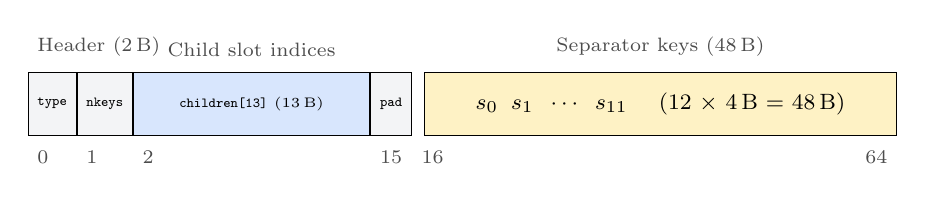
\begin{tikzpicture}[
  box/.style={draw, minimum height=0.8cm, font=\footnotesize, anchor=west},
  lbl/.style={font=\scriptsize, text=gray!60!black},
]
  \node[box, fill=headercolor, minimum width=0.5cm] (type) at (0,0) {\tiny\code{type}};
  \node[box, fill=headercolor, minimum width=0.6cm, right=0pt of type] (nk) {\tiny\code{nkeys}};
  \node[box, fill=ptrcolor!20, minimum width=3.0cm, right=0pt of nk] (ch)
    {\tiny\code{children[13]} (\SI{13}{\byte})};
  \node[box, fill=headercolor, minimum width=0.4cm, right=0pt of ch] (pad) {\tiny\code{pad}};
  \node[box, fill=simdblk!50, minimum width=6.0cm, right=0.15cm of pad] (keys)
    {$s_0 \;\; s_1 \;\; \cdots \;\; s_{11}$ \quad (12 $\times$ \SI{4}{\byte} = \SI{48}{\byte})};

  % Byte offsets
  \node[lbl, below=2pt of type.south west, anchor=north west] {0};
  \node[lbl, below=2pt of type.south east, anchor=north west] {1};
  \node[lbl, below=2pt of nk.south east, anchor=north west] {2};
  \node[lbl, below=2pt of ch.south east, anchor=north west] {15};
  \node[lbl, below=2pt of pad.south east, anchor=north west] {16};
  \node[lbl, below=2pt of keys.south east, anchor=north east] {64};

  % Labels
  \node[lbl, above=2pt of type.north west, anchor=south west] {Header (\SI{2}{\byte})};
  \node[lbl, above=2pt of ch.north, anchor=south] {Child slot indices};
  \node[lbl, above=2pt of keys.north, anchor=south] {Separator keys (\SI{48}{\byte})};
\end{tikzpicture}
\caption{\textbf{CL internal sub-node layout (\code{mt\_cl\_inode\_t}, \SI{64}{\byte}).}
  \code{type} = \code{MT\_CL\_INTERNAL} (1 byte), \code{nkeys} = number
  of separator keys (1 byte), \code{children[13]} = slot indices
  (13 bytes, each a \code{uint8\_t} in range 1--63), 1 byte padding,
  then up to 12 sorted \code{int32\_t} separator keys.
  Total: $1 + 1 + 13 + 1 + 48 = 64$ bytes.}
\label{fig:cl-inode-layout}
\end{figure}

Children are \code{uint8\_t} slot indices (1--63) pointing to other CL
sub-nodes within the same page.  The routing semantics follow the
standard B\textsuperscript{+} tree convention: child $c_i$ leads to
keys in range $[s_{i-1}, s_i)$, with $c_0$ covering $(-\infty, s_0)$
and $c_n$ covering $[s_{n-1}, +\infty)$.

Maximum: 12 separator keys, 13 children.  Minimum: 7 children
($\ceil{13/2}$), 6 separator keys.

\subsection{Page Header (\code{mt\_page\_header\_t})}
\label{sec:page-header}

Slot~0 of every leaf page is the page header, which occupies one
cache line:

\begin{figure}[H]
\centering
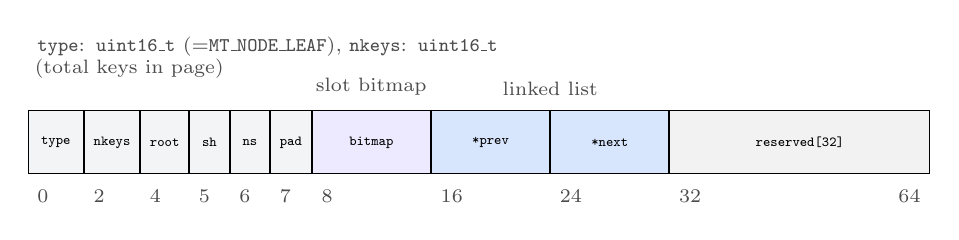
\begin{tikzpicture}[
  box/.style={draw, minimum height=0.8cm, font=\footnotesize, anchor=west},
  lbl/.style={font=\scriptsize, text=gray!60!black},
]
  % First row: fixed fields
  \node[box, fill=headercolor, minimum width=0.7cm] (type) at (0,0) {\tiny\code{type}};
  \node[box, fill=headercolor, minimum width=0.7cm, right=0pt of type] (nkeys) {\tiny\code{nkeys}};
  \node[box, fill=headercolor, minimum width=0.5cm, right=0pt of nkeys] (rs) {\tiny\code{root}};
  \node[box, fill=headercolor, minimum width=0.5cm, right=0pt of rs] (sh) {\tiny\code{sh}};
  \node[box, fill=headercolor, minimum width=0.5cm, right=0pt of sh] (ns) {\tiny\code{ns}};
  \node[box, fill=headercolor, minimum width=0.5cm, right=0pt of ns] (pd) {\tiny\code{pad}};
  \node[box, fill=clblk!30, minimum width=1.5cm, right=0pt of pd] (bm) {\tiny\code{bitmap}};
  \node[box, fill=ptrcolor!20, minimum width=1.5cm, right=0pt of bm] (prev) {\tiny\code{*prev}};
  \node[box, fill=ptrcolor!20, minimum width=1.5cm, right=0pt of prev] (next) {\tiny\code{*next}};
  \node[box, fill=gray!10, minimum width=3.3cm, right=0pt of next] (rsv)
    {\tiny\code{reserved[32]}};

  % Byte offsets
  \node[lbl, below=2pt of type.south west, anchor=north west] {0};
  \node[lbl, below=2pt of nkeys.south west, anchor=north west] {2};
  \node[lbl, below=2pt of rs.south west, anchor=north west] {4};
  \node[lbl, below=2pt of sh.south west, anchor=north west] {5};
  \node[lbl, below=2pt of ns.south west, anchor=north west] {6};
  \node[lbl, below=2pt of pd.south west, anchor=north west] {7};
  \node[lbl, below=2pt of bm.south west, anchor=north west] {8};
  \node[lbl, below=2pt of prev.south west, anchor=north west] {16};
  \node[lbl, below=2pt of next.south west, anchor=north west] {24};
  \node[lbl, below=2pt of rsv.south west, anchor=north west] {32};
  \node[lbl, below=2pt of rsv.south east, anchor=north east] {64};

  % Labels
  \node[lbl, above=8pt of type.north west, anchor=south west, text width=6cm]
    {\code{type}: \code{uint16\_t} (=\code{MT\_NODE\_LEAF}),
     \code{nkeys}: \code{uint16\_t} (total keys in page)};
  \node[lbl, above=2pt of bm.north, anchor=south] {slot bitmap};
  \node[lbl, above=2pt of prev.north east, anchor=south] {linked list};
\end{tikzpicture}
\caption{\textbf{Page header layout (\code{mt\_page\_header\_t}, \SI{64}{\byte}).}
  \code{type} (\SI{2}{\byte}): outer node type.
  \code{nkeys} (\SI{2}{\byte}): total keys in page.
  \code{root\_slot} (\SI{1}{\byte}): CL slot index of sub-tree root.
  \code{sub\_height} (\SI{1}{\byte}): 0 = single CL leaf.
  \code{nslots\_used} (\SI{1}{\byte}): allocated CL slot count.
  \code{slot\_bitmap} (\SI{8}{\byte}): bits 1--63 track allocation.
  \code{prev}/\code{next} (\SI{8}{\byte} each): leaf linked list.
  \code{reserved} (\SI{32}{\byte}): padding to \SI{64}{\byte}.}
\label{fig:page-header}
\end{figure}

\subsection{Leaf Page Layout}
\label{sec:page-layout}

Each leaf page is a \SI{4}{\kilo\byte} (\SI{4096}{\byte}) region
divided into 64 cache-line slots of \SI{64}{\byte} each:

\begin{figure}[H]
\centering
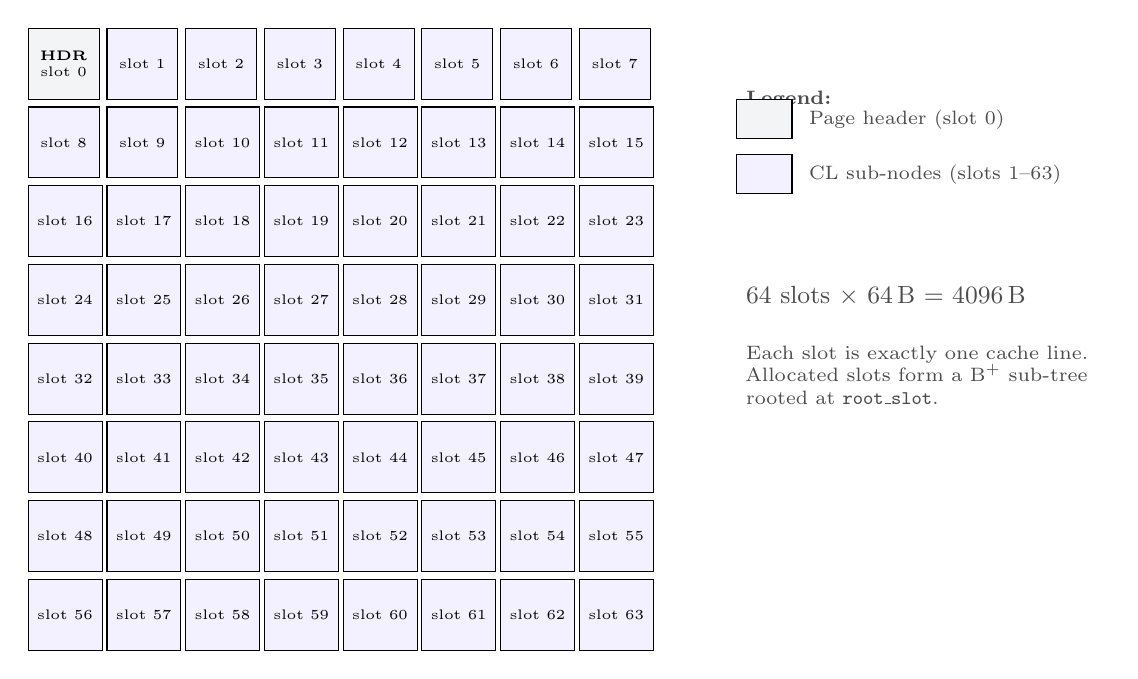
\begin{tikzpicture}[
  slot/.style={draw, minimum width=0.9cm, minimum height=0.9cm,
               font=\tiny, align=center, anchor=south west},
  lbl/.style={font=\scriptsize, text=gray!60!black},
]
  % Draw 8 rows of 8 slots = 64 slots
  \foreach \row in {0,...,7} {
    \foreach \col in {0,...,7} {
      \pgfmathtruncatemacro{\idx}{\row * 8 + \col}
      \ifnum\idx=0
        \node[slot, fill=headercolor] (s\idx)
          at ({\col * 1.0}, {-\row * 1.0}) {\textbf{HDR}\\slot 0};
      \else
        \ifnum\idx<64
          \node[slot, fill=clblk!20] (s\idx)
            at ({\col * 1.0}, {-\row * 1.0}) {slot \idx};
        \fi
      \fi
    }
  }

  % Legend
  \node[lbl, anchor=west] at (9, 0) {\textbf{Legend:}};
  \node[slot, fill=headercolor, minimum width=0.7cm, minimum height=0.5cm]
    at (9, -0.5) {};
  \node[lbl, anchor=west] at (9.8, -0.25) {Page header (slot 0)};
  \node[slot, fill=clblk!20, minimum width=0.7cm, minimum height=0.5cm]
    at (9, -1.2) {};
  \node[lbl, anchor=west] at (9.8, -0.95) {CL sub-nodes (slots 1--63)};

  % Page boundary
  \node[lbl, anchor=west, font=\small] at (9, -2.5)
    {64 slots $\times$ \SI{64}{\byte} $=$ \SI{4096}{\byte}};
  \node[lbl, anchor=west, text width=4.5cm] at (9, -3.5)
    {Each slot is exactly one cache line. Allocated slots form a B\textsuperscript{+}
     sub-tree rooted at \code{root\_slot}.};

\end{tikzpicture}
\caption{\textbf{Leaf page layout.}
  A \SI{4}{\kilo\byte} page contains 64 cache-line slots.  Slot~0 is the
  page header.  Slots 1--63 are available for CL sub-nodes.  Allocation
  is tracked by a \code{uint64\_t} bitmap in the header (bits 1--63).
  Free slots have type \code{MT\_CL\_FREE}; allocated slots are either
  CL leaves or CL internals forming the intra-page B\textsuperscript{+}
  sub-tree.}
\label{fig:page-layout}
\end{figure}

\subsection{Capacity Analysis}
\label{sec:capacity}

The maximum number of keys per page depends on the sub-tree height:

\begin{table}[H]
\centering
\caption{\textbf{Page capacity by sub-tree height.}  Each CL leaf holds
  up to 15 keys; each CL internal has up to 13 children.}
\label{tab:capacity}
\small
\begin{tabular}{@{}ccccl@{}}
\toprule
\textbf{Sub-height} & \textbf{CL Internals} & \textbf{CL Leaves} & \textbf{Slots Used} & \textbf{Max Keys} \\
\midrule
0 & 0  & 1   & 1  & $1 \times 15 = 15$ \\
1 & 1  & 13  & 14 & $13 \times 15 = 195$ \\
2 & 5--6 & 57 & 62--63 & $57 \times 15 = 855$ \\
\bottomrule
\end{tabular}
\end{table}

At sub-height~2, the page is nearly fully utilised (63 of 63 usable slots).
For a \SI{4}{\kilo\byte} page, the practical maximum is approximately 855
keys---somewhat more than the 511-key flat array of the previous design,
though the effective limit depends on fill factor after splits.

The sub-tree grows in height as CL leaves fill and split, allocating CL
internal nodes from free slots.  When no free slots remain, the page
signals \code{MT\_PAGE\_FULL} to the outer tree, which splits the page.

\subsection{Outer B\textsuperscript{+} Tree Internal Node
  (\code{mt\_inode\_t})}
\label{sec:inode}

Internal nodes store sorted keys and child pointers in a conventional
B\textsuperscript{+} layout, unchanged from the classical design:

\begin{equation}
  \underbrace{p_0}_{\text{child}_0} \;
  k_1 \;
  \underbrace{p_1}_{\text{child}_1} \;
  k_2 \;
  \underbrace{p_2}_{\text{child}_2} \;
  \cdots \;
  k_m \;
  \underbrace{p_m}_{\text{child}_m}
\label{eq:inode-layout}
\end{equation}

The maximum number of keys per internal node:
\begin{equation}
  \underbrace{16}_{\text{header}} + 4m + 8(m+1) \le 4096
  \quad\Longrightarrow\quad
  m \le 339
\label{eq:inode-capacity}
\end{equation}

\begin{figure}[H]
\centering
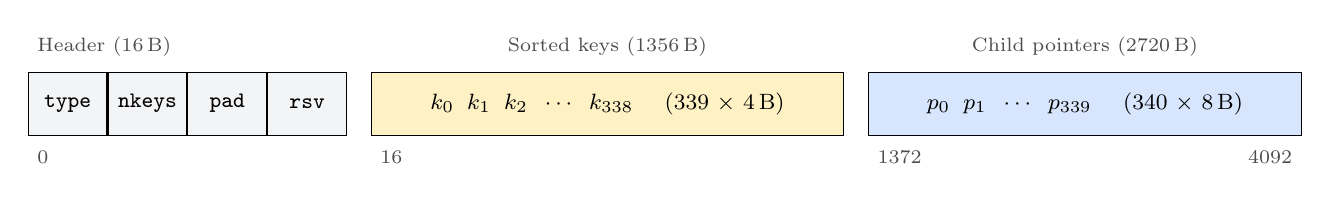
\begin{tikzpicture}[
  box/.style={draw, minimum height=0.8cm, font=\footnotesize, anchor=west},
  lbl/.style={font=\scriptsize, text=gray!60!black},
]
  % Header
  \node[box, fill=headercolor, minimum width=1.0cm] (type) at (0,0) {\code{type}};
  \node[box, fill=headercolor, minimum width=1.0cm, right=0pt of type] (nkeys) {\code{nkeys}};
  \node[box, fill=headercolor, minimum width=1.0cm, right=0pt of nkeys] (pad) {\code{pad}};
  \node[box, fill=headercolor, minimum width=1.0cm, right=0pt of pad] (rsv) {\code{rsv}};

  % Keys
  \node[box, fill=simdblk!50, minimum width=6.0cm, right=0.3cm of rsv] (keys)
    {$k_0 \;\; k_1 \;\; k_2 \;\; \cdots \;\; k_{338}$ \quad (339 $\times$ \SI{4}{\byte})};

  % Children
  \node[box, fill=ptrcolor!20, minimum width=5.5cm, right=0.3cm of keys] (children)
    {$p_0 \;\; p_1 \;\; \cdots \;\; p_{339}$ \quad (340 $\times$ \SI{8}{\byte})};

  % Byte offsets
  \node[lbl, below=2pt of type.south west, anchor=north west] {0};
  \node[lbl, below=2pt of keys.south west, anchor=north west] {16};
  \node[lbl, below=2pt of children.south west, anchor=north west] {1372};
  \node[lbl, below=2pt of children.south east, anchor=north east] {4092};

  % Labels
  \node[lbl, above=2pt of type.north west, anchor=south west] {Header (\SI{16}{\byte})};
  \node[lbl, above=2pt of keys.north, anchor=south] {Sorted keys (\SI{1356}{\byte})};
  \node[lbl, above=2pt of children.north, anchor=south] {Child pointers (\SI{2720}{\byte})};
\end{tikzpicture}
\caption{\textbf{Internal node (\code{mt\_inode\_t}) memory layout.}
  The header (\SI{16}{\byte}) contains the node type, key count, and padding.
  The sorted key array holds up to 339 \code{int32\_t} keys.  The child
  pointer array holds up to 340 \code{mt\_node\_t*} pointers.
  Total: $16 + 1356 + 2720 = 4092$ bytes.}
\label{fig:inode-layout}
\end{figure}

Internal node search uses SIMD-accelerated linear scan for $\le 32$
keys (loading 4 keys per \code{\_mm\_loadu\_si128}, comparing via
\code{\_mm\_cmpgt\_epi32}) and falls back to scalar binary search
for larger nodes.


% ══════════════════════════════════════════════════════════════════
\section{Page-Level Sub-Tree Operations}
\label{sec:page-ops}

This section describes operations on the CL B\textsuperscript{+} sub-tree
within a single leaf page.  All operations are confined to the
\SI{4}{\kilo\byte} page boundary.

\subsection{Intra-Page Sub-Tree Structure}
\label{sec:subtree-structure}

The CL sub-nodes within a page form a standard B\textsuperscript{+}
sub-tree:

\begin{figure}[H]
\centering
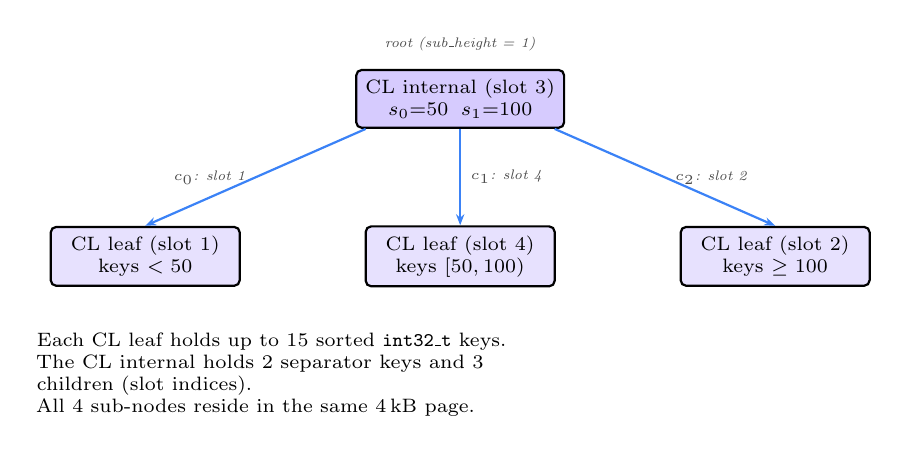
\begin{tikzpicture}[
  clnode/.style={draw, thick, rounded corners=2pt,
                 minimum width=2.4cm, minimum height=0.7cm,
                 font=\scriptsize, align=center},
  cleaf/.style={clnode, fill=clblk!40},
  cinode/.style={clnode, fill=clblk!70},
  arr/.style={-{Stealth[length=4pt]}, thick, ptrcolor},
  lbl/.style={font=\tiny\itshape, text=gray!60!black},
]
  % Root CL internal (sub-height 1 example)
  \node[cinode] (r) at (0, 0)
    {CL internal (slot 3)\\$s_0{=}50 \;\; s_1{=}100$};
  \node[lbl, above=3pt of r] {root (sub\_height = 1)};

  % CL leaves
  \node[cleaf] (l0) at (-4.0, -2.0)
    {CL leaf (slot 1)\\keys $< 50$};
  \node[cleaf] (l1) at (0, -2.0)
    {CL leaf (slot 4)\\keys $[50, 100)$};
  \node[cleaf] (l2) at (4.0, -2.0)
    {CL leaf (slot 2)\\keys $\ge 100$};

  % Arrows
  \draw[arr] (r.south) ++(-1.2, 0) -- (l0.north)
    node[midway, lbl, left] {$c_0$: slot 1};
  \draw[arr] (r.south) -- (l1.north)
    node[midway, lbl, right] {$c_1$: slot 4};
  \draw[arr] (r.south) ++(1.2, 0) -- (l2.north)
    node[midway, lbl, right] {$c_2$: slot 2};

  % Capacity annotation
  \node[font=\scriptsize, anchor=west, text width=6cm] at (-5.5, -3.5) {%
    Each CL leaf holds up to 15 sorted \code{int32\_t} keys.\\
    The CL internal holds 2 separator keys and 3 children (slot indices).\\
    All 4 sub-nodes reside in the same \SI{4}{\kilo\byte} page.};

\end{tikzpicture}
\caption{\textbf{Intra-page CL sub-tree (sub-height 1).}
  The root is a CL internal node at slot~3, with two separator keys
  (50, 100) and three child slot indices pointing to CL leaf sub-nodes.
  Slot indices are \code{uint8\_t} values in the range 1--63.}
\label{fig:cl-subtree}
\end{figure}

\subsection{Search}
\label{sec:page-search}

Searching within a page traverses the CL sub-tree from root to CL leaf:

\begin{enumerate}[nosep]
  \item Start at the sub-tree root slot (\code{header.root\_slot}).
  \item At each CL internal node, perform an SIMD-accelerated scan of
    the separator keys (up to 12 keys, scanned 4 at a time via
    \code{\_mm\_cmpgt\_epi32}).  This yields the child index $c_i$;
    follow \code{children[$c_i$]} to the next slot.
  \item Repeat for \code{sub\_height} levels until reaching a CL leaf.
  \item In the CL leaf, perform an SIMD predecessor scan of the sorted
    keys (up to 15 keys, scanned 4 at a time).  Return the largest
    key $\le q$.
\end{enumerate}

\begin{figure}[H]
\centering
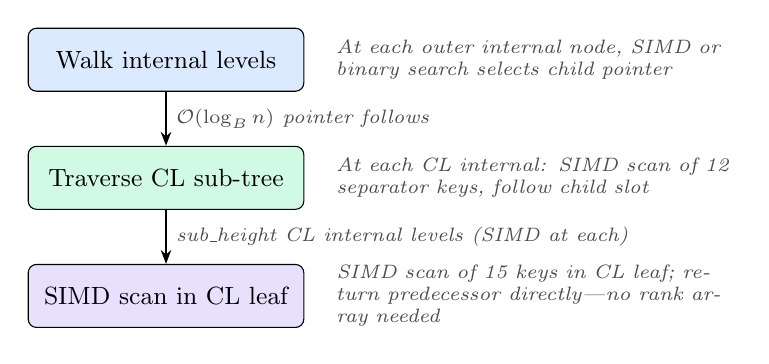
\begin{tikzpicture}[
  stepbox/.style={draw, rounded corners=3pt, minimum width=3.5cm,
               minimum height=0.8cm, font=\small, align=center},
  arrow/.style={-{Stealth[length=5pt]}, thick},
  lbl/.style={font=\scriptsize\itshape, text=gray!60!black},
]
  \node[stepbox, fill=inodecolor] (s1) at (0, 0) {Walk internal levels};
  \node[stepbox, fill=leafcolor] (s2) at (0, -1.5) {Traverse CL sub-tree};
  \node[stepbox, fill=clblk!40] (s3) at (0, -3.0) {SIMD scan in CL leaf};

  \draw[arrow] (s1) -- (s2) node[midway, right, lbl]
    {$\Oh(\log_B n)$ pointer follows};
  \draw[arrow] (s2) -- (s3) node[midway, right, lbl]
    {sub\_height CL internal levels (SIMD at each)};

  \node[lbl, right=0.3cm of s1, text width=5cm]
    {At each outer internal node, SIMD or binary search selects child pointer};
  \node[lbl, right=0.3cm of s2, text width=5cm]
    {At each CL internal: SIMD scan of 12 separator keys, follow child slot};
  \node[lbl, right=0.3cm of s3, text width=5cm]
    {SIMD scan of 15 keys in CL leaf; return predecessor directly---no rank
     array needed};
\end{tikzpicture}
\caption{\textbf{Search procedure.}
  The search is $\Oh(\log_B n + \text{sub\_height})$, where each
  sub-tree level does $\Oh(1)$ SIMD work (scanning $\le 15$ keys).}
\label{fig:search-procedure}
\end{figure}

Because CL leaves store keys in sorted order, the predecessor is found
directly---there is no need for a separate \code{sorted\_rank[]} array
or sorted-key extraction, as was required by the old FAST-blocked design.

If the predecessor is not in the current CL leaf (i.e., the query is
smaller than all keys in this leaf), the search walks left through the
sub-tree path to find the rightmost key of the preceding CL leaf.

\subsection{Insert}
\label{sec:page-insert}

Insertion into a page proceeds as follows:

\begin{enumerate}[nosep]
  \item \textbf{Navigate}: Traverse the CL sub-tree to the target CL leaf.
  \item \textbf{Insert into CL leaf}: If the CL leaf has room ($< 15$
    keys), binary-search for the insertion point, shift keys right
    (\code{memmove} of at most \SI{60}{\byte}), and insert.  Done.
  \item \textbf{CL leaf full}: Split the CL leaf.  Allocate a new CL
    slot from the page bitmap.  Move the upper half of keys to the new
    CL leaf.  The separator (first key of the right half) is pushed up
    to the parent CL internal.
  \item \textbf{CL internal full}: If the parent CL internal has no room
    ($= 12$ separator keys), split it too.  The median separator is
    promoted further up.
  \item \textbf{Sub-tree root split}: If the split propagates to the
    sub-tree root, allocate a new CL internal as the new root, increasing
    \code{sub\_height} by 1.
  \item \textbf{Page full}: If no CL slots are available for the split,
    return \code{MT\_PAGE\_FULL}.  The outer tree handles this by
    splitting the entire page.
\end{enumerate}

\begin{figure}[H]
\centering
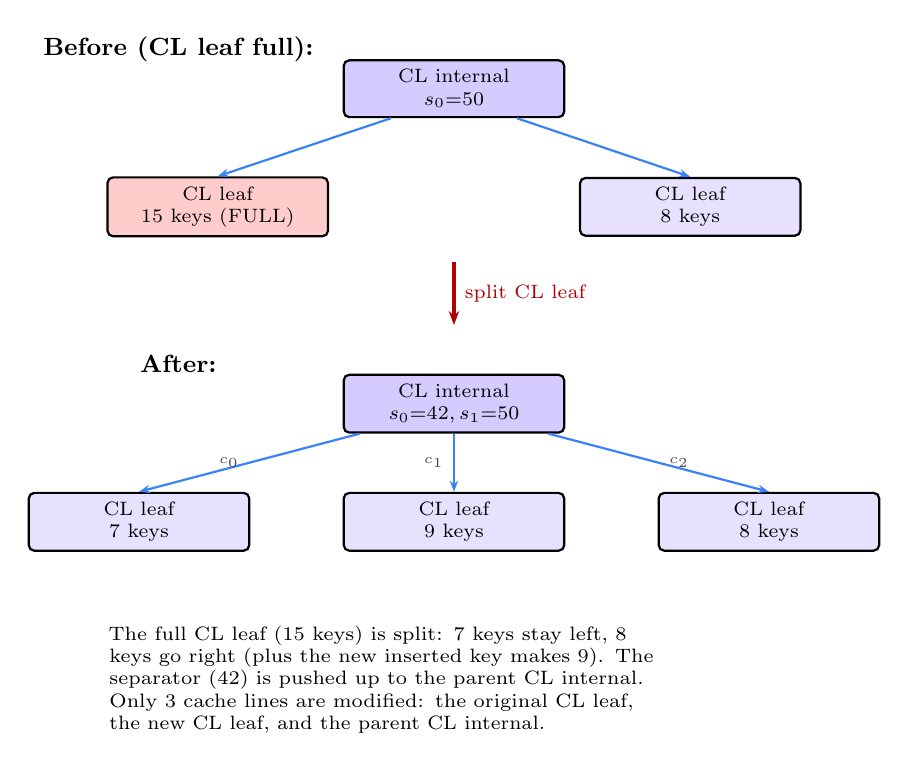
\begin{tikzpicture}[
  clnode/.style={draw, thick, rounded corners=2pt,
                 minimum width=2.8cm, minimum height=0.7cm,
                 font=\scriptsize, align=center},
  cleaf/.style={clnode, fill=clblk!40},
  cinode/.style={clnode, fill=clblk!70},
  arr/.style={-{Stealth[length=4pt]}, thick, ptrcolor},
  splitarr/.style={-{Stealth[length=5pt]}, very thick, red!70!black},
  lbl/.style={font=\tiny\itshape, text=gray!60!black},
]
  % Before: full CL leaf
  \node[font=\small\bfseries] at (-5.5, 2.0) {Before (CL leaf full):};
  \node[cinode] (p1) at (-2, 1.5) {CL internal\\$s_0{=}50$};
  \node[cleaf, fill=red!20] (f1) at (-5, 0) {CL leaf\\15 keys (FULL)};
  \node[cleaf] (f2) at (1, 0) {CL leaf\\8 keys};
  \draw[arr] (p1.south) ++(-0.8, 0) -- (f1.north);
  \draw[arr] (p1.south) ++(0.8, 0) -- (f2.north);

  % Arrow
  \draw[splitarr] (-2, -0.7) -- (-2, -1.5)
    node[midway, right, font=\scriptsize, red!70!black] {split CL leaf};

  % After: split
  \node[font=\small\bfseries] at (-5.5, -2.0) {After:};
  \node[cinode] (p2) at (-2, -2.5) {CL internal\\$s_0{=}42, s_1{=}50$};
  \node[cleaf] (a1) at (-6, -4.0) {CL leaf\\7 keys};
  \node[cleaf] (a2) at (-2, -4.0) {CL leaf\\9 keys};
  \node[cleaf] (a3) at (2, -4.0) {CL leaf\\8 keys};
  \draw[arr] (p2.south) ++(-1.2, 0) -- (a1.north) node[midway, lbl, left] {$c_0$};
  \draw[arr] (p2.south) -- (a2.north) node[midway, lbl, left] {$c_1$};
  \draw[arr] (p2.south) ++(1.2, 0) -- (a3.north) node[midway, lbl, right] {$c_2$};

  \node[font=\scriptsize, text width=7cm, anchor=north west] at (-6.5, -5.2) {%
    The full CL leaf (15 keys) is split: 7 keys stay left, 8 keys go right
    (plus the new inserted key makes 9).  The separator (42) is pushed up
    to the parent CL internal.  Only 3 cache lines are modified: the
    original CL leaf, the new CL leaf, and the parent CL internal.};
\end{tikzpicture}
\caption{\textbf{CL leaf split during insert.}
  When a CL leaf overflows, it is split and the separator is promoted to
  the parent CL internal node.  All operations are within the same
  \SI{4}{\kilo\byte} page.}
\label{fig:cl-split}
\end{figure}

\paragraph{Cost.}
Inserting into a CL leaf costs $\Oh(15)$ (shift at most 15 keys).
A CL leaf split touches 2 CL leaves and 1 CL internal.  In the worst
case, a split propagates through \code{sub\_height} CL internal levels,
each requiring $\Oh(12)$ key shifts.  Total per-page insert cost:
$\Oh(\text{sub\_height} \times 15)$.

\subsection{Delete}
\label{sec:page-delete}

Deletion mirrors insertion, with underflow handling:

\begin{enumerate}[nosep]
  \item \textbf{Navigate and remove}: Traverse to the CL leaf, delete the
    key (\code{memmove} left).
  \item \textbf{Check underflow}: If the CL leaf has $\ge 7$ keys
    ($\floor{15/2}$), done.
  \item \textbf{Redistribute}: Try borrowing a key from a sibling CL leaf
    (via the parent CL internal).  If a sibling has $> 7$ keys, move one
    key and update the parent separator.
  \item \textbf{Merge}: If no sibling can spare keys, merge with a sibling.
    Copy all keys into one CL leaf, free the other slot (clear its bitmap
    bit), and remove the separator from the parent CL internal.
  \item \textbf{Propagate}: If the parent CL internal underflows ($< 7$
    children), apply redistribute or merge at the CL internal level
    (key rotation through the grandparent).  Continue up to the sub-tree
    root.
  \item \textbf{Root collapse}: If the sub-tree root has 0 keys and 1 child
    after a merge, replace the root with its child, decreasing
    \code{sub\_height}.
  \item \textbf{Page underflow}: If the total key count falls below the
    page minimum, return \code{MT\_UNDERFLOW}.  The outer tree handles
    page-level redistribute or merge.
\end{enumerate}

\begin{figure}[H]
\centering
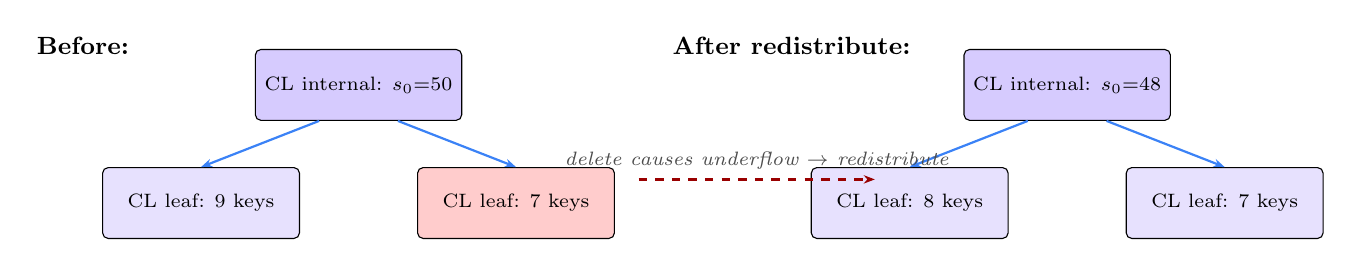
\begin{tikzpicture}[
  node/.style={draw, rounded corners=2pt, minimum height=0.9cm,
               font=\scriptsize, align=center},
  cleaf/.style={node, fill=clblk!40, minimum width=2.5cm},
  cinode/.style={node, fill=clblk!70, minimum width=2.5cm},
  arrow/.style={-{Stealth[length=4pt]}, thick},
  lbl/.style={font=\scriptsize\itshape, text=gray!60!black},
]
  % Before
  \node[font=\small\bfseries] at (-0.5, 2.5) {Before:};
  \node[cinode] (p1) at (3, 2.0) {CL internal: $s_0{=}50$};
  \node[cleaf]  (a1) at (1.0, 0.5) {CL leaf: 9 keys};
  \node[cleaf, fill=red!20]  (b1) at (5.0, 0.5) {CL leaf: 7 keys};
  \draw[arrow, ptrcolor] (p1.south) ++(-0.5,0) -- (a1.north);
  \draw[arrow, ptrcolor] (p1.south) ++(0.5,0) -- (b1.north);

  % After redistribute
  \node[font=\small\bfseries] at (8.5, 2.5) {After redistribute:};
  \node[cinode] (p2) at (12, 2.0) {CL internal: $s_0{=}48$};
  \node[cleaf]  (a2) at (10.0, 0.5) {CL leaf: 8 keys};
  \node[cleaf]  (b2) at (14.0, 0.5) {CL leaf: 7 keys};
  \draw[arrow, ptrcolor] (p2.south) ++(-0.5,0) -- (a2.north);
  \draw[arrow, ptrcolor] (p2.south) ++(0.5,0) -- (b2.north);

  \draw[arrow, red!60!black, dashed, thick] (b1.east) ++(0.3,0.3) -- ++(3.0,0)
    node[midway, above, lbl] {delete causes underflow $\to$ redistribute};
\end{tikzpicture}
\caption{\textbf{CL leaf redistribute during delete.}
  After deletion, the right CL leaf has 6 keys (below minimum of 7).
  One key is moved from the left sibling (9 keys, above minimum), and
  the parent separator is updated.  Only 3 cache lines are touched.}
\label{fig:cl-redistribute}
\end{figure}

\begin{figure}[H]
\centering
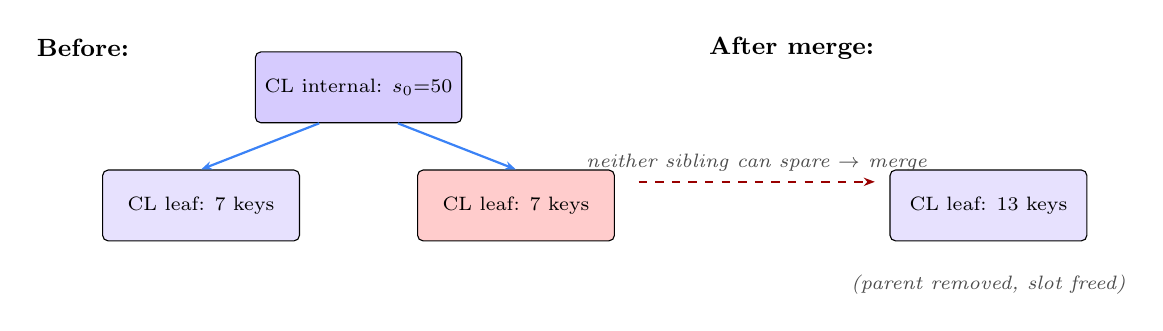
\begin{tikzpicture}[
  node/.style={draw, rounded corners=2pt, minimum height=0.9cm,
               font=\scriptsize, align=center},
  cleaf/.style={node, fill=clblk!40, minimum width=2.5cm},
  cinode/.style={node, fill=clblk!70, minimum width=2.5cm},
  deadnode/.style={draw, dashed, rounded corners=2pt, minimum height=0.7cm,
                   font=\scriptsize, text=gray, fill=gray!10, minimum width=2.0cm},
  arrow/.style={-{Stealth[length=4pt]}, thick},
  lbl/.style={font=\scriptsize\itshape, text=gray!60!black},
]
  % Before
  \node[font=\small\bfseries] at (-0.5, 2.5) {Before:};
  \node[cinode] (p1) at (3, 2.0) {CL internal: $s_0{=}50$};
  \node[cleaf]  (a1) at (1.0, 0.5) {CL leaf: 7 keys};
  \node[cleaf, fill=red!20]  (b1) at (5.0, 0.5) {CL leaf: 7 keys};
  \draw[arrow, ptrcolor] (p1.south) ++(-0.5,0) -- (a1.north);
  \draw[arrow, ptrcolor] (p1.south) ++(0.5,0) -- (b1.north);

  % After merge
  \node[font=\small\bfseries] at (8.5, 2.5) {After merge:};
  \node[cleaf] (ab) at (11, 0.5) {CL leaf: 13 keys};
  \node[lbl] at (11, -0.5) {(parent removed, slot freed)};

  \draw[arrow, red!60!black, dashed, thick] (b1.east) ++(0.3,0.3) -- ++(3.0,0)
    node[midway, above, lbl] {neither sibling can spare $\to$ merge};
\end{tikzpicture}
\caption{\textbf{CL leaf merge during delete.}
  Both CL leaves are at minimum occupancy (7 keys each).  They are merged
  into a single CL leaf (13 keys), the other slot is freed back to the
  bitmap, and the separator is removed from the parent CL internal.}
\label{fig:cl-merge}
\end{figure}

\subsection{Page Split}
\label{sec:page-split}

When a page runs out of free CL slots, it must be split:

\begin{enumerate}[nosep]
  \item \textbf{Extract}: Perform an in-order traversal of the CL
    sub-tree to extract all keys in sorted order.
  \item \textbf{Divide}: Split the sorted keys at the midpoint.
  \item \textbf{Bulk load}: Rebuild each half into a fresh page via
    \code{mt\_page\_bulk\_load}, which fills CL leaves sequentially and
    builds CL internal levels bottom-up.
  \item \textbf{Return separator}: The first key of the right page becomes
    the separator pushed to the outer B\textsuperscript{+} tree parent.
\end{enumerate}

Page split is the only operation that touches all keys in a page ($\Oh(n)$
where $n$ is the page key count).  It occurs only when the page is
completely full (all 63 CL slots allocated), which is infrequent during
normal operation.

\subsection{Bulk Load}
\label{sec:page-bulk-load}

Bulk loading constructs an optimal CL sub-tree from a sorted key array:

\begin{enumerate}[nosep]
  \item \textbf{Partition}: Divide keys evenly across CL leaves, each
    holding up to 15 keys.
  \item \textbf{Fill CL leaves}: Allocate a CL slot for each leaf, copy
    keys directly.
  \item \textbf{Build internal levels}: Group CL leaves into parents of up
    to 13 children each.  If more than one parent is needed, repeat at the
    next level until a single root remains.
  \item \textbf{Set header}: Record \code{root\_slot}, \code{sub\_height},
    \code{nkeys}, and \code{nslots\_used}.
\end{enumerate}

This produces a balanced, densely packed sub-tree in $\Oh(n)$ time.


% ══════════════════════════════════════════════════════════════════
\section{Outer B\textsuperscript{+} Tree Operations}
\label{sec:outer-ops}

The outer B\textsuperscript{+} tree uses standard pointer-based
navigation, with leaf pages as its leaf nodes and conventional internal
nodes (\code{mt\_inode\_t}).

\subsection{Bulk Load}
\label{sec:outer-bulk-load}

\begin{figure}[H]
\centering
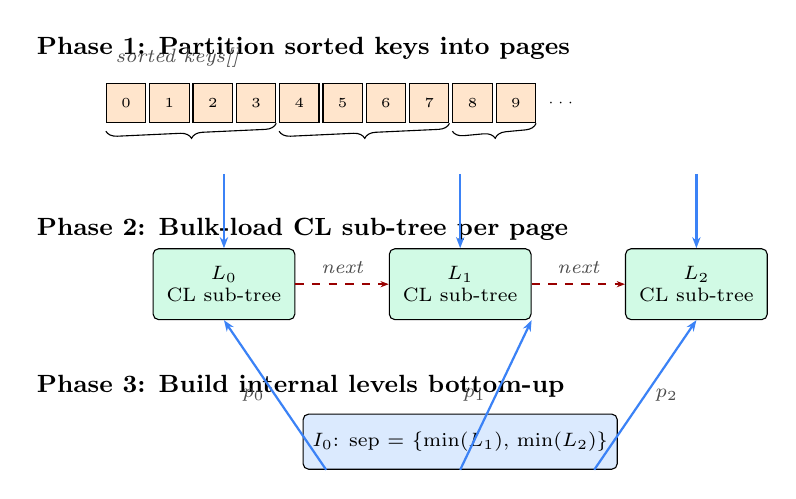
\begin{tikzpicture}[
  leaf/.style={draw, fill=leafcolor, rounded corners=2pt,
               minimum width=1.8cm, minimum height=0.9cm,
               font=\scriptsize, align=center},
  inode/.style={draw, fill=inodecolor, rounded corners=2pt,
                minimum width=2.5cm, minimum height=0.7cm,
                font=\scriptsize, align=center},
  arr/.style={draw, minimum width=0.5cm, minimum height=0.5cm,
              font=\tiny, anchor=west},
  arrow/.style={-{Stealth[length=4pt]}, thick, ptrcolor},
  lbl/.style={font=\scriptsize\itshape, text=gray!60!black},
  phase/.style={font=\small\bfseries, anchor=west},
]

  % Phase 1
  \node[phase] at (-6, 3.5) {Phase 1: Partition sorted keys into pages};
  \foreach \i/\k in {0/0, 1/1, 2/2, 3/3, 4/4, 5/5, 6/6, 7/7, 8/8, 9/9} {
    \node[arr, fill=orange!20] (a\i) at ({-5.0 + \i * 0.55}, 2.8) {\k};
  }
  \node[font=\tiny] at ({-5.0 + 10*0.55 + 0.3}, 2.8) {$\cdots$};
  \node[lbl, above=2pt of a0.north west, anchor=south west] {sorted keys[]};

  \draw[decorate, decoration={brace, amplitude=4pt, mirror}]
    (a0.south west) ++(0,-0.1) -- (a3.south east) ++(0,-0.1);
  \draw[decorate, decoration={brace, amplitude=4pt, mirror}]
    (a4.south west) ++(0,-0.1) -- (a7.south east) ++(0,-0.1);
  \draw[decorate, decoration={brace, amplitude=4pt, mirror}]
    (a8.south west) ++(0,-0.1) -- (a9.south east) ++(0,-0.1);

  % Phase 2
  \node[phase] at (-6, 1.2) {Phase 2: Bulk-load CL sub-tree per page};
  \node[leaf] (l0) at (-3.5, 0.5) {$L_0$\\CL sub-tree};
  \node[leaf] (l1) at (-0.5, 0.5) {$L_1$\\CL sub-tree};
  \node[leaf] (l2) at (2.5, 0.5) {$L_2$\\CL sub-tree};

  \draw[arrow] (-3.5, 1.9) -- (l0.north);
  \draw[arrow] (-0.5, 1.9) -- (l1.north);
  \draw[arrow] (2.5, 1.9) -- (l2.north);

  % Leaf links
  \draw[-{Stealth[length=3pt]}, red!60!black, dashed, thick]
    (l0.east) -- (l1.west) node[midway, above, lbl] {next};
  \draw[-{Stealth[length=3pt]}, red!60!black, dashed, thick]
    (l1.east) -- (l2.west) node[midway, above, lbl] {next};

  % Phase 3
  \node[phase] at (-6, -0.8) {Phase 3: Build internal levels bottom-up};
  \node[inode] (i0) at (-0.5, -1.5) {$I_0$: sep = \{min($L_1$), min($L_2$)\}};

  \draw[arrow] (i0.south west) ++(0.3, 0) -- (l0.south)
    node[midway, left, lbl] {$p_0$};
  \draw[arrow] (i0.south) -- (l1.south east)
    node[midway, left, lbl] {$p_1$};
  \draw[arrow] (i0.south east) ++(-0.3, 0) -- (l2.south)
    node[midway, right, lbl] {$p_2$};

\end{tikzpicture}
\caption{\textbf{Bulk load construction.}
  \textbf{Phase~1}: Sorted keys are partitioned across pages.
  \textbf{Phase~2}: Each page's CL sub-tree is bulk-loaded via
  \code{mt\_page\_bulk\_load}.  Pages are linked via \code{prev}/\code{next}.
  \textbf{Phase~3}: Internal nodes are built bottom-up with separator keys
  (the minimum key of each non-first child page).}
\label{fig:bulk-load}
\end{figure}

\subsection{Point Query and Predecessor Search}
\label{sec:outer-search}

A predecessor search for query $q$ combines outer tree traversal with
intra-page sub-tree search:

\begin{enumerate}[nosep]
  \item Walk from the root through internal levels ($\Oh(\log_B n)$
    pointer follows, with SIMD search at each internal node).
  \item At the target leaf page, call \code{mt\_page\_search\_key},
    which traverses the CL sub-tree (\code{sub\_height} levels of SIMD
    scans) to find the predecessor.
  \item If the predecessor is not found in this page (the query is
    smaller than all keys in this page), the outer tree follows the
    \code{prev} pointer to check the preceding leaf.
\end{enumerate}

\subsection{Insert}
\label{sec:outer-insert}

\begin{enumerate}[nosep]
  \item \textbf{Find leaf page}: Walk from root to the target page,
    recording the path.
  \item \textbf{Page insert}: Call \code{mt\_page\_insert}, which
    navigates the CL sub-tree and inserts into the appropriate CL leaf,
    splitting CL sub-nodes as needed.
  \item \textbf{If \code{MT\_OK}}: Done.  Only individual CL sub-nodes
    were modified.
  \item \textbf{If \code{MT\_DUPLICATE}}: Return false (key exists).
  \item \textbf{If \code{MT\_PAGE\_FULL}}: The page has no free CL slots.
    Split the entire page via \code{mt\_page\_split}: extract all keys,
    divide in half, bulk-load each half.  Push the separator to the parent
    internal node.  If the parent overflows, split it too (standard
    B\textsuperscript{+} tree internal split).
\end{enumerate}

\begin{figure}[H]
\centering
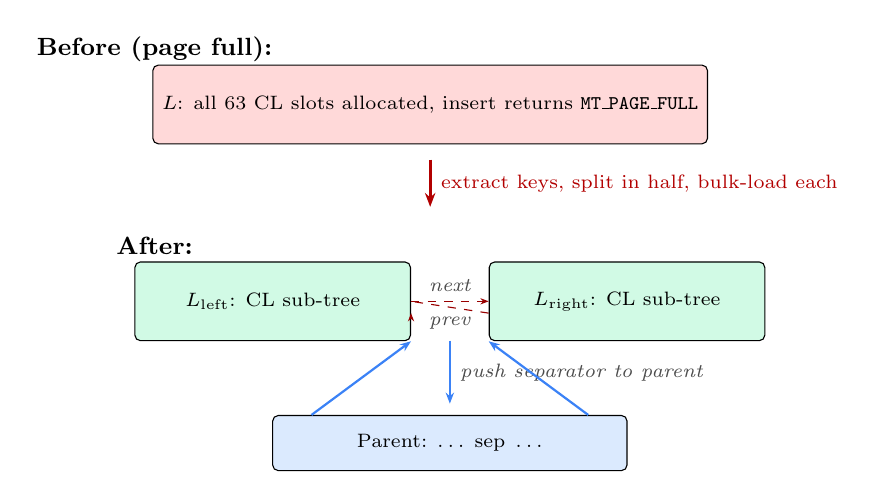
\begin{tikzpicture}[
  leaf/.style={draw, fill=leafcolor, rounded corners=2pt,
               minimum width=4.5cm, minimum height=1.0cm,
               font=\scriptsize, align=center},
  inode/.style={draw, fill=inodecolor, rounded corners=2pt,
                minimum width=4.5cm, minimum height=0.7cm,
                font=\scriptsize, align=center},
  arrow/.style={-{Stealth[length=4pt]}, thick},
  lbl/.style={font=\scriptsize\itshape, text=gray!60!black},
  splitarrow/.style={-{Stealth[length=5pt]}, very thick, red!70!black},
]
  % Before
  \node[font=\small\bfseries] at (-3.5, 3.2) {Before (page full):};
  \node[leaf, minimum width=7cm, fill=red!15] (full) at (0, 2.5)
    {$L$: all 63 CL slots allocated, insert returns \code{MT\_PAGE\_FULL}};

  \draw[splitarrow] (0, 1.8) -- (0, 1.2)
    node[midway, right, font=\scriptsize, red!70!black]
    {extract keys, split in half, bulk-load each};

  % After
  \node[font=\small\bfseries] at (-3.5, 0.7) {After:};
  \node[leaf, minimum width=3.5cm] (left) at (-2.0, 0.0)
    {$L_{\text{left}}$: CL sub-tree};
  \node[leaf, minimum width=3.5cm] (right) at (2.5, 0.0)
    {$L_{\text{right}}$: CL sub-tree};

  \draw[-{Stealth[length=3pt]}, red!60!black, dashed]
    (left.east) -- (right.west) node[midway, above, lbl] {next};
  \draw[-{Stealth[length=3pt]}, red!60!black, dashed]
    (right.west) ++(0,-0.15) -- (left.east |- right.west) ++(0,-0.15)
    node[midway, below, lbl] {prev};

  \draw[arrow, ptrcolor] (0.25, -0.5) -- (0.25, -1.3)
    node[midway, right, lbl] {push separator to parent};
  \node[inode] (parent) at (0.25, -1.8)
    {Parent: $\ldots\; \text{sep} \;\ldots$};
  \draw[arrow, ptrcolor] (parent.north west) ++(0.5,0) -- (left.south east);
  \draw[arrow, ptrcolor] (parent.north east) ++(-0.5,0) -- (right.south west);

\end{tikzpicture}
\caption{\textbf{Page split during insertion.}
  When a page is full and cannot accommodate a CL sub-node split, all keys
  are extracted, divided in half, and each half is bulk-loaded into a fresh
  page.  The separator is pushed to the parent internal node.}
\label{fig:page-split}
\end{figure}

\subsection{Delete}
\label{sec:outer-delete}

\begin{enumerate}[nosep]
  \item \textbf{Find and remove}: Walk from root to page.  Call
    \code{mt\_page\_delete}, which navigates the CL sub-tree, deletes
    from the CL leaf, and handles CL-level redistribute/merge.
  \item \textbf{If \code{MT\_OK}}: Done.
  \item \textbf{If \code{MT\_NOT\_FOUND}}: Return false.
  \item \textbf{If \code{MT\_UNDERFLOW}}: The page has too few keys.
    Try redistributing keys from a sibling page (extract both pages'
    sorted keys, redistribute evenly, bulk-load both).  If redistribution
    is not possible, merge with a sibling (combine keys, bulk-load one
    page, free the other).  Remove the separator from the parent.
    Propagate upward if the parent underflows.
  \item \textbf{Root collapse}: If the root internal node has 0 keys and
    1 child, replace it with its child.
\end{enumerate}

\subsection{Range Scan (Iteration)}
\label{sec:iteration}

An iterator is positioned at a leaf page and extracts its sorted keys
into a buffer (via in-order traversal of the CL sub-tree).  Advancing
yields keys from the buffer; when exhausted, the iterator follows the
\code{next} pointer and extracts the next page's keys.

\begin{figure}[H]
\centering
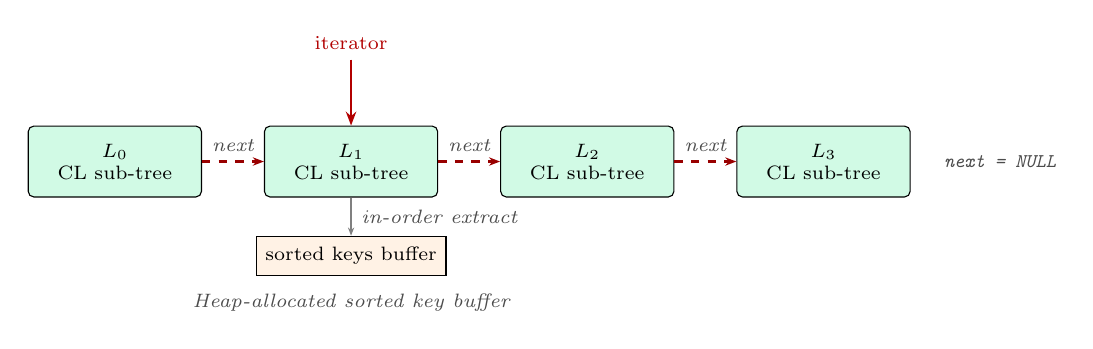
\begin{tikzpicture}[
  leaf/.style={draw, fill=leafcolor, rounded corners=2pt,
               minimum width=2.2cm, minimum height=0.9cm,
               font=\scriptsize, align=center},
  arrow/.style={-{Stealth[length=4pt]}, thick, red!60!black, dashed},
  lbl/.style={font=\scriptsize\itshape, text=gray!60!black},
  cursor/.style={draw, thick, red!70!black, -{Stealth[length=5pt]}},
]
  \node[leaf] (l0) at (0, 0)    {$L_0$\\CL sub-tree};
  \node[leaf] (l1) at (3.0, 0)  {$L_1$\\CL sub-tree};
  \node[leaf] (l2) at (6.0, 0)  {$L_2$\\CL sub-tree};
  \node[leaf] (l3) at (9.0, 0)  {$L_3$\\CL sub-tree};

  \draw[arrow] (l0.east) -- (l1.west) node[midway, above, lbl] {next};
  \draw[arrow] (l1.east) -- (l2.west) node[midway, above, lbl] {next};
  \draw[arrow] (l2.east) -- (l3.west) node[midway, above, lbl] {next};

  \node[font=\scriptsize, red!70!black] (iter) at (3.0, 1.5) {iterator};
  \draw[cursor] (iter.south) -- (l1.north);

  \node[draw, fill=orange!10, minimum width=2.2cm, minimum height=0.5cm,
        font=\scriptsize] (buf) at (3.0, -1.2) {sorted keys buffer};
  \draw[-{Stealth[length=3pt]}, thick, gray] (l1.south) -- (buf.north)
    node[midway, right, lbl] {in-order extract};

  \node[lbl, below=3pt of buf] {Heap-allocated sorted key buffer};
  \node[lbl, right=0.3cm of l3] {\code{next = NULL}};
\end{tikzpicture}
\caption{\textbf{Iterator traversal via leaf linked list.}
  The iterator extracts a page's sorted keys by in-order traversal of its
  CL sub-tree, then yields keys from the buffer.  When exhausted, it
  follows \code{next} to the adjacent page.}
\label{fig:iterator}
\end{figure}


% ══════════════════════════════════════════════════════════════════
\section{Complexity Analysis}
\label{sec:complexity}

Table~\ref{tab:complexity} summarises the asymptotic costs of matryoshka
tree operations.  Let $n$ denote the total key count, $B$ the maximum
keys per page (approximately 855 at sub-height 2), $b = 15$ the CL leaf
capacity, $f = 13$ the CL internal fanout, $F = 340$ the outer internal
fanout, $h_s$ the intra-page sub-tree height, and $h_o$ the outer tree
height.

\begin{table}[H]
\centering
\caption{\textbf{Operation costs.}
  $h_o = \Oh(\log_F(n/B))$, $h_s \le 2$ for \SI{4}{\kilo\byte} pages.}
\label{tab:complexity}
\small
\begin{tabular}{@{}lll@{}}
\toprule
\textbf{Operation} & \textbf{Asymptotic Cost} & \textbf{Notes} \\
\midrule
Bulk load       & $\Oh(n)$ & Bottom-up construction \\
Point search    & $\Oh(h_o + h_s)$ & $h_o$ pointer follows + $h_s$ CL internal scans + 1 CL leaf scan \\
Predecessor     & $\Oh(h_o + h_s)$ & Same as point search (no rank array needed) \\
Insert (no split) & $\Oh(h_o + h_s \cdot b)$ & Navigate + CL operations \\
Insert (page split) & $\Oh(B + h_o)$ & Extract + rebuild both halves + parent update \\
Delete (no merge) & $\Oh(h_o + h_s \cdot b)$ & Navigate + CL operations \\
Delete (page merge) & $\Oh(B + h_o)$ & Extract + rebuild + parent update \\
Range scan      & $\Oh(h_o + m)$ & $h_o$ for initial seek, $m$ keys scanned \\
Iteration (next)& $\Oh(1)$ amortised & $\Oh(B)$ per page transition (re-extract) \\
\bottomrule
\end{tabular}
\end{table}

\paragraph{Concrete numbers.}
For $n = 10{,}000{,}000$ keys with pages at sub-height 2 ($B \approx 855$):
\begin{itemize}[nosep]
  \item Pages: $\ceil{10^7 / 855} \approx 11{,}700$ leaf pages.
  \item Outer tree height: $h_o = \ceil{\log_{340}(11{,}700)} \approx 2$.
  \item Sub-tree height: $h_s = 2$ (1 root CL internal + up to 5 CL
    internals + 57 CL leaves).
  \item Total cache lines per search: 2 outer internal nodes (1 CL each) + 3 CL
    sub-nodes (root + internal + leaf) = 5 cache-line accesses.
\end{itemize}

\paragraph{Comparison with old design.}
The old FAST-blocked flat array design required $\Oh(B) = \Oh(511)$ work
per insertion or deletion (full extract, sort, and FAST-layout rebuild).
The new CL sub-tree design requires $\Oh(h_s \times b) = \Oh(2 \times 15)
= \Oh(30)$ in the common case (no page split).  This is a roughly
\textbf{15--20$\times$ reduction} in per-modification cost, at comparable
search performance.


% ══════════════════════════════════════════════════════════════════
\section{Cache Behaviour Analysis}
\label{sec:cache}

The matryoshka tree's performance depends critically on how its data
structures interact with the CPU cache hierarchy.

\subsection{Within a Page (CL Sub-Tree)}

Each CL sub-node is exactly \SI{64}{\byte}---one cache line.  Navigating
the CL sub-tree from root to leaf touches exactly $h_s + 1$ cache lines
(one per CL internal level plus the CL leaf).  For sub-height 2, this is
3 cache lines, all within the same \SI{4}{\kilo\byte} page.

Within each CL sub-node, the SIMD scan processes 4 keys per SSE2
comparison.  A CL leaf of 15 keys requires $\ceil{15/4} = 4$ SIMD
comparisons in the worst case.  A CL internal of 12 separators requires
$\ceil{12/4} = 3$ comparisons.

Because all CL sub-nodes reside in the same page, they share the same
TLB entry.  Traversing the CL sub-tree incurs zero TLB misses after the
initial page access.

\subsection{Between Pages (Outer B\textsuperscript{+} Tree)}

Each pointer follow between outer tree nodes may incur a TLB miss if
the target resides on a different virtual page.  Since nodes are
page-aligned, each node occupies exactly one TLB entry.  The TLB cost
per search is bounded by $h_o + 1$ (one per internal level plus the
leaf page), typically 2--3 for trees up to $10^8$ keys.

\subsection{Comparison with Old Design}

The old FAST-blocked design stored up to 511 keys in a flat array within
each leaf, requiring $\ceil{9/2} = 5$ SIMD block traversals per search
(9 levels of binary tree, 2 levels per SIMD block).  The new CL sub-tree
design requires $h_s + 1 = 3$ cache-line accesses with SIMD scans of
12--15 keys each.  The number of SIMD \emph{instructions} is comparable
(5 old vs.\ 3--4 new per sub-tree level), but each new access touches a
full cache line worth of sorted keys rather than a 3-key SIMD block,
giving better data density per cache-line fetch.

\subsection{Comparison with Pure FAST}

Pure FAST trees eliminate all pointer follows by storing the entire index
in a contiguous array.  For trees fitting in L2/L3 cache, FAST achieves
higher raw search throughput.  The matryoshka tree trades a small number
of pointer follows ($h_o = 1$--2 per search) for the ability to modify
the tree efficiently---$\Oh(h_s \times b)$ per insert/delete versus
$\Oh(n)$ for FAST's full rebuild.


% ══════════════════════════════════════════════════════════════════
\section{Implementation Notes}
\label{sec:impl}

\subsection{Arena Allocator}

Leaf pages are allocated from a \SI{2}{\mebi\byte} arena allocator
(\code{mt\_allocator\_t}).  Each arena is a superpage-sized region:

\begin{lstlisting}
/* Try huge page allocation first. */
void *p = mmap(NULL, arena_size, PROT_READ | PROT_WRITE,
               MAP_PRIVATE | MAP_ANONYMOUS | MAP_HUGETLB, -1, 0);
if (p == MAP_FAILED) {
    /* Fallback: aligned allocation + transparent huge page hint. */
    posix_memalign(&p, arena_size, arena_size);
    madvise(p, arena_size, MADV_HUGEPAGE);
}
\end{lstlisting}

Each arena is subdivided into page-sized slots tracked by a
\code{uint64\_t} bitmap (one bit per page).  Allocation scans the bitmap
for a free bit via \code{\_\_builtin\_ctzll}; deallocation clears the bit.
When all arenas are full, a new arena is allocated.

Co-locating leaf pages within the same superpage-aligned arena reduces TLB
misses during sequential scans: pages allocated during bulk load or
adjacent inserts end up in the same \SI{2}{\mebi\byte} region, covered by
a single TLB entry.

Internal nodes are allocated via \code{posix\_memalign} with
\SI{4096}{\byte} alignment (one page each, outside the arena).

\subsection{Slot Allocation within a Page}

CL slot allocation within a leaf page uses the \code{slot\_bitmap} field
in the page header.  Bit~0 is always set (it represents the header slot).
Bits 1--63 represent CL sub-node slots:

\begin{lstlisting}
/* Allocate a CL slot: find lowest clear bit in range 1-63. */
uint64_t avail = ~page->header.slot_bitmap & ~1ULL;
if (avail == 0) return 0;  /* page full */
int slot = __builtin_ctzll(avail);
page->header.slot_bitmap |= (1ULL << slot);
\end{lstlisting}

Deallocation clears the corresponding bit.  This provides $\Oh(1)$
allocation and deallocation.

\subsection{Compilation Constants}

\begin{table}[H]
\centering
\caption{\textbf{Compile-time constants} defined in \code{matryoshka\_internal.h}.}
\label{tab:constants}
\small
\begin{tabular}{@{}lrl@{}}
\toprule
\textbf{Constant} & \textbf{Value} & \textbf{Description} \\
\midrule
\code{MT\_PAGE\_SIZE}      & 4096  & Page size in bytes \\
\code{MT\_CL\_SIZE}        & 64    & Cache-line size in bytes \\
\code{MT\_CL\_KEY\_CAP}    & 15    & Keys per CL leaf \\
\code{MT\_CL\_MIN\_KEYS}   & 7     & Minimum CL leaf occupancy ($\floor{15/2}$) \\
\code{MT\_CL\_SEP\_CAP}    & 12    & Separator keys per CL internal \\
\code{MT\_CL\_CHILD\_CAP}  & 13    & Children per CL internal \\
\code{MT\_CL\_MIN\_CHILDREN}& 7    & Minimum CL internal children ($\ceil{13/2}$) \\
\code{MT\_PAGE\_SLOTS}     & 63    & Usable CL slots per page (slots 1--63) \\
\code{MT\_MAX\_IKEYS}      & 339   & Max keys per outer internal node \\
\code{MT\_MIN\_IKEYS}      & 169   & Min keys per outer internal node ($\floor{339/2}$) \\
\code{MT\_MAX\_LEVELS}     & 8     & Maximum hierarchy levels \\
\code{MT\_KEY\_MAX}         & $2^{31}-1$ & Sentinel value (\code{INT32\_MAX}) \\
\bottomrule
\end{tabular}
\end{table}

\subsection{Runtime Hierarchy Configuration}

The \code{mt\_hierarchy\_t} structure stores per-tree configuration:

\begin{table}[H]
\centering
\caption{\textbf{Runtime hierarchy fields} in \code{mt\_hierarchy\_t}.}
\label{tab:hierarchy-fields}
\small
\begin{tabular}{@{}lll@{}}
\toprule
\textbf{Field} & \textbf{Default} & \textbf{Description} \\
\midrule
\code{leaf\_alloc}       & 4096 & Leaf page allocation size \\
\code{cl\_key\_cap}      & 15   & Keys per CL leaf \\
\code{cl\_sep\_cap}      & 12   & Separator keys per CL internal \\
\code{cl\_child\_cap}    & 13   & Children per CL internal \\
\code{page\_slots}       & 63   & Usable CL slots per page \\
\code{page\_max\_keys}   & $\sim$855 & Max keys per page (sub-height dependent) \\
\code{min\_page\_keys}   & varies & Minimum page occupancy for outer tree \\
\code{min\_cl\_keys}     & 7    & Minimum CL leaf occupancy \\
\code{min\_cl\_children} & 7    & Minimum CL internal children \\
\bottomrule
\end{tabular}
\end{table}

\subsection{Limitations and Future Work}

\begin{itemize}[nosep]
  \item \textbf{Concurrency}: No locking or versioning is implemented.
    Optimistic lock coupling~\cite{lehman1981efficient} or epoch-based
    reclamation would be needed for concurrent access.

  \item \textbf{Variable-length keys}: The current design is specialised
    for 32-bit integers.  Supporting variable-length keys would require
    indirection or key normalisation, similar to Masstree's approach.

  \item \textbf{Superpage-level nesting}: The current design nests only
    two levels (CL sub-tree within page, pages within outer tree).  A
    future extension could add a third nesting level: a B\textsuperscript{+}
    sub-tree of pages within a \SI{2}{\mebi\byte} superpage, further
    reducing TLB misses for very large datasets.

  \item \textbf{Architecture-specific tuning}: Factory functions currently
    target x86-64 with SSE2.  Adding presets for ARM NEON, AVX2 (8 keys
    per comparison), and AVX-512 (16 keys per comparison) would broaden
    applicability and increase the effective SIMD scan width.
\end{itemize}


% ══════════════════════════════════════════════════════════════════
\section{Summary}
\label{sec:summary}

The matryoshka tree is a B\textsuperscript{+} tree in which each leaf page
contains a B\textsuperscript{+} sub-tree of cache-line-sized sub-nodes.
This matryoshka nesting---trees within trees at every level of the memory
hierarchy---delivers both efficient search and efficient modification:

\begin{enumerate}[nosep]
  \item \textbf{SIMD-accelerated intra-page search}: The CL sub-tree is
    navigated via SIMD scans of 12--15 keys at each level, touching
    $h_s + 1$ cache lines (typically 2--3) per leaf page.

  \item \textbf{Per-key modifications without flat-array rebuild}: Insert
    and delete operate on individual CL sub-nodes---splitting, merging,
    and redistributing cache-line-sized structures---costing
    $\Oh(h_s \times 15)$ per modification versus the old $\Oh(511)$
    flat rebuild.  This is a $\sim$15--20$\times$ improvement.

  \item \textbf{Standard B\textsuperscript{+} tree outer structure}:
    The outer tree uses pointer-based navigation with page-level splits
    and merges, supporting $\Oh(\log_B n)$ structural modifications.

  \item \textbf{Eager deletion at every level}: Jannink's
    redistribute/merge algorithm operates at both the CL sub-tree level
    and the outer tree level, maintaining minimum occupancy invariants
    throughout.

  \item \textbf{Arena allocation with huge pages}: Leaf pages are
    co-located in \SI{2}{\mebi\byte} arenas for TLB locality.

  \item \textbf{Efficient range scans}: A doubly-linked leaf list enables
    sequential iteration; an in-order traversal of each page's CL
    sub-tree extracts sorted keys.
\end{enumerate}

The nested architecture---SIMD registers inside cache-line sub-nodes
inside page-sized sub-trees inside the outer B\textsuperscript{+} tree---mirrors
the memory hierarchy itself, giving the structure its name: like a
matryoshka doll, each level contains a smaller, self-similar structure
within.


% ══════════════════════════════════════════════════════════════════
\begin{thebibliography}{99}

\bibitem{bayer1972organization}
R.~Bayer and E.~McCreight.
\newblock Organization and maintenance of large ordered indexes.
\newblock \emph{Acta Informatica}, 1(3):173--189, 1972.

\bibitem{comer1979ubiquitous}
D.~Comer.
\newblock The ubiquitous {B}-tree.
\newblock \emph{ACM Computing Surveys}, 11(2):121--137, 1979.

\bibitem{graefe2011modern}
G.~Graefe.
\newblock Modern {B}-tree techniques.
\newblock \emph{Foundations and Trends in Databases}, 3(4):203--402, 2011.

\bibitem{hankins2003effect}
R.~A. Hankins and J.~M. Patel.
\newblock Effect of node size on the performance of cache-conscious
  {B}\textsuperscript{+}-trees.
\newblock In \emph{Proc.\ ACM SIGMETRICS}, pages 283--294, 2003.

\bibitem{kim2010fast}
C.~Kim, J.~Chhugani, N.~Satish, E.~Sedlar, A.~D. Nguyen, T.~Kaldewey,
  V.~W. Lee, S.~A. Brandt, and P.~Dubey.
\newblock {FAST}: {Fast} architecture sensitive tree search on modern {CPUs}
  and {GPUs}.
\newblock In \emph{Proc.\ ACM SIGMOD}, pages 339--350, 2010.

\bibitem{lehman1981efficient}
P.~L. Lehman and S.~B. Yao.
\newblock Efficient locking for concurrent operations on {B}-trees.
\newblock \emph{ACM Trans.\ Database Systems}, 6(4):650--670, 1981.

\bibitem{leis2013adaptive}
V.~Leis, A.~Kemper, and T.~Neumann.
\newblock The adaptive radix tree: {ARTful} indexing for main-memory databases.
\newblock In \emph{Proc.\ IEEE ICDE}, pages 38--49, 2013.

\bibitem{mao2012cache}
Y.~Mao, E.~Kohler, and R.~T. Morris.
\newblock Cache craftiness for fast multicore key-value storage.
\newblock In \emph{Proc.\ ACM EuroSys}, pages 183--196, 2012.

\bibitem{rao1999cache}
J.~Rao and K.~A. Ross.
\newblock Cache conscious indexing for decision-support in main memory.
\newblock In \emph{Proc.\ VLDB}, pages 78--89, 1999.

\bibitem{rao2000making}
J.~Rao and K.~A. Ross.
\newblock Making {B}\textsuperscript{+}-trees cache conscious in main memory.
\newblock In \emph{Proc.\ ACM SIGMOD}, pages 475--486, 2000.

\bibitem{schlegel2009kary}
B.~Schlegel, R.~Gemulla, and W.~Lehner.
\newblock {K}-ary search on modern processors.
\newblock In \emph{Proc.\ DaMoN Workshop}, pages 52--60, 2009.

\bibitem{jannink1995implementing}
J.~Jannink.
\newblock Implementing deletion in {B}\textsuperscript{+}-trees.
\newblock \emph{ACM SIGMOD Record}, 24(1):33--38, 1995.

\bibitem{zhou2002implementing}
J.~Zhou and K.~A. Ross.
\newblock Implementing database operations using {SIMD} instructions.
\newblock In \emph{Proc.\ ACM SIGMOD}, pages 145--156, 2002.

\end{thebibliography}

\end{document}
